\documentclass[10pt,journal,compsoc]{IEEEtran}
% \documentclass[9.5pt,journal,compsoc]{IEEEtran}
\IEEEoverridecommandlockouts
\hyphenation{op-tical net-works semi-conduc-tor}
\usepackage{orcidlink}
\usepackage{amsmath,amssymb,amsfonts}
\usepackage{amsthm}
\usepackage{algorithmic}
\usepackage{algorithm}
\usepackage{graphicx}
\usepackage{textcomp}
\usepackage{xcolor}
\usepackage{booktabs}
\usepackage{multirow}
\usepackage{mathtools}
\usepackage{url}
\usepackage{hyperref}
\usepackage{subcaption}
\usepackage{svg}
\usepackage{tikz}
\usepackage{array}
\usepackage{pgfplots}
\pgfplotsset{compat=1.18}
\usetikzlibrary{shapes,arrows,positioning,fit,calc}
\usepackage{balance}
\usepackage{threeparttable}
\usepackage{pifont}
\usepackage{mdframed}
\usepackage{pgffor}
\mdfdefinestyle{schemestyle}{linewidth=0.8pt,linecolor=black!70,backgroundcolor=black!3,
  innertopmargin=5pt,innerbottommargin=6pt,innerleftmargin=7pt,innerrightmargin=7pt,
  skipabove=7pt,skipbelow=7pt,roundcorner=2pt}
\newenvironment{scheme}[1]{\par\begin{mdframed}[style=schemestyle]\textbf{Scheme.}\ \textit{#1}\par\vspace{2pt}\small}{\end{mdframed}}
\newenvironment{gamebox}[1]{\par\begin{mdframed}[style=schemestyle]\textbf{Game.}\ \textit{#1}\par\vspace{2pt}\small}{\end{mdframed}}
\graphicspath{{Figure/figures/}{figures/}{../results/figures/}{results/figures/}{./}}

\newtheorem{definition}{Definition}
\newtheorem{theorem}{Theorem}
\newtheorem{lemma}{Lemma}

\newcolumntype{C}[1]{>{\centering\arraybackslash}p{#1}}
\newcolumntype{L}[1]{>{\raggedright\arraybackslash}p{#1}}

\hyphenation{block-chain}
\newtheorem{proposition}{Proposition}
\newtheorem{corollary}{Corollary}
\renewcommand{\topfraction}{0.95}
\renewcommand{\bottomfraction}{0.95}
\renewcommand{\textfraction}{0.05}
\renewcommand{\floatpagefraction}{0.9}
\renewcommand{\dbltopfraction}{0.95}
\renewcommand{\dblfloatpagefraction}{0.9}
\begin{document}

\title{TrustCircuit: Blockchain-Orchestrated Privacy-Preserving Data Circulation with Verifiable Compliance}

\author{Bao~Huynh\,\orcidlink{0009-0008-8773-0482},
        Tuan-Dung~Tran\,\orcidlink{0000-0003-1156-7072},
        Dang Van~Huynh\, \orcidlink{0000-0002-2314-4934}
        and~Van-Hau~Pham\,\orcidlink{0000-0003-3147-3356}%
\thanks{Bao Huynh, Tuan-Dung Tran, Dang Van~Huynh and Van-Hau Pham are with the University of Information Technology, Vietnam National University, Ho Chi Minh City, Vietnam.}
\thanks{Email: 23520104@gm.uit.edu.vn, dungtrt@uit.edu.vn, danghv@uit.edu.vn, haupv@uit.edu.vn}}

\markboth{IEEE Transactions on Network Science and Engineering}%
{Huynh \MakeLowercase{\textit{et al.}}: TrustCircuit: Blockchain-Orchestrated Privacy-Preserving Data Circulation}

\IEEEtitleabstractindextext{%
\begin{abstract}
Organizations increasingly reuse sensitive data across administrative boundaries, but granting access is not enough: each subsequent computation must remain tied to the approved policy, privacy budget, execution context, and audit record. Existing systems typically secure these decisions separately, allowing evidence from different stages to be valid in isolation without proving that it belongs to the same data-use request. We present TrustCircuit, a blockchain-orchestrated protocol that turns each data use into a request-indexed state transition. Its central contribution is the Verifiable Compliance Protocol (VCP), which binds the active policy, reserved and consumed privacy budget, validated execution context, released-result commitment, replay-prevention nullifier, and audit transition into one settlement statement. Building this lifecycle requires reconciling three mismatches: real-valued privacy accounting with deterministic ledger state, platform-specific attestation with compact proof inputs, and policy evolution with circuit-specific setup. TrustCircuit addresses them through conservative budget translation, a canonical attestation statement, and a policy-parameterized proof relation reusable within a fixed policy family. VCP targets the encoded lifecycle relation; native attestation validation and arbitrary program semantics remain outside the proof. The canonical two-rule VCP relation has $40{,}161$ constraints and $24$ public inputs. Across $30$ retained runs after two warm-ups, Groth16 proving requires $1.007$ s on average, produces a $256$-byte A/B/C ABI object ($723$-byte median snarkjs JSON), and consumes $374{,}753$ gas at the median for isolated verification. On Base Sepolia, $30$ real-proof settlements through the final eight-contract stack consume $554{,}496$ gas at the median and reach inclusion in $2.964$ s.
\end{abstract}

\begin{IEEEkeywords}
Blockchain, Privacy-Preserving Data Circulation, Trusted Execution Environment (TEE), Differential Privacy, Zero-Knowledge Proof (ZKP), Verifiable Compliance, Decentralized Data Sharing.
\end{IEEEkeywords}}


% make the title area
\maketitle

\IEEEdisplaynontitleabstractindextext
\IEEEpeerreviewmaketitle

\IEEEraisesectionheading{
\section{Introduction}\label{sec:introduction}}

Cross-organizational analytics increasingly depends on the repeated use of sensitive data across healthcare, finance, digital services, and connected infrastructures. Recent blockchain-based systems have strengthened accountable authorization, provenance, and data exchange while retaining sensitive payloads outside the ledger~\cite{hoang2024promark,sun2022verifiable}. Confidential-computing research has advanced scalable personal-data analytics and auditable service identities through protected execution and transparent attestation~\cite{de2025covault,delignat2025transparent}. In parallel, recent verification systems have produced machine-checkable evidence for differential-privacy mechanisms, federated updates, and complex inference workloads~\cite{zhang2025robust,qu2025zkgpt,zhou2025vprivkv}.

These developments broaden the assurance available at individual stages of data use, but governance increasingly concerns the complete operation rather than only its admission. The EU AI Act and related auditing frameworks emphasize traceability of the governing rules, execution conditions, risk controls, and resulting records~\cite{euaiact2024,mokander2022conformity}. Ledger-based data-sharing systems commonly record ownership, authorization, transformation, or marketplace accountability~\cite{sun2022verifiable,hoang2024promark}. Confidential-computing platforms instead establish protected execution and attested service identity~\cite{brossard2023private,de2025covault}. Verifiable-privacy systems provide strong evidence for particular reports or privacy mechanisms, but generally maintain a narrower application-specific state boundary~\cite{bontekoe2024efficient,zhou2025vprivkv}.

This separation becomes consequential when the same data asset serves multiple requests over time. A policy decision valid at admission may no longer match the active policy at settlement. A reserved privacy budget may differ from the expenditure reported after computation, while an otherwise valid result commitment, attestation statement, or proof may belong to another request or policy version. Existing computation-specific proofs authenticate reports, model updates, or inference statements, whereas request admission, cumulative budget state, replay control, and audit settlement commonly remain external to their proof relation~\cite{wei2025verifiable,bellachia2025verifbfl,qu2025zkgpt}.

This paper presents \textbf{TrustCircuit}, a blockchain orchestrated protocol that represents every approved data-use operation as a guarded, request-indexed state transition. A request progresses through authorization, privacy-budget reservation, confidential execution, evidence validation, proof verification, and settlement. Acceptance requires the policy version, approved function, dataset snapshot, execution context, released-result commitment, privacy expenditure, nullifier, and audit outcome to refer to the same asset, consumer, and request.

Supporting this lifecycle introduces three cross-layer problems. First, real-valued privacy expenditure computed by an off-chain accountant must enter deterministic ledger state without under-reporting cumulative disclosure. Second, platform-native attestation evidence must be translated into a compact authenticated context that remains linked to both the arithmetic proof and the current request state. Third, policy amendments should update the accepted policy instance without forcing circuit recompilation and a new circuit-specific setup whenever the dimensions of the policy family remain unchanged.

TrustCircuit addresses these problems through conservative fixed-point budget enforcement, a dual-domain attestation bridge, and a policy-parameterized compliance relation. Its \emph{Verifiable Compliance Protocol} (VCP) binds encoded policy satisfaction, requested and actual privacy expenditure, execution and result commitments, request identity, nullifier state, and audit transition through one shared interface. The settlement contract verifies that this interface matches the active asset, policy, reservation, validator statement, and ledger state before atomically consuming the request budget and nullifier.

The VCP statement is scoped to the encoded lifecycle relation. Native certificate-chain validation is performed by the attestation-validation layer, whose authenticated output is bound to the proof and settlement state. Full program semantics and the internal randomness of the differential-privacy mechanism remain governed by the validated execution context. Consequently, an accepted transaction establishes agreement across the lifecycle fields that determine settlement, preventing independently valid evidence from different requests, results, policy versions, or budget states from forming an accepted circulation event.

The main contributions are as follows:

\begin{itemize}
    \item We formulate data circulation as a guarded request-indexed transition system with atomic budget consumption, nullifier use, and audit settlement, and establish request-trace serializability and one-shot completion.

    \item We construct VCP as a fiber-product relation whose policy, budget, execution-context, result, nullifier, and audit predicates must agree on one request-bound interface.

    \item We develop a conservative fixed-point interface for off-chain R\'enyi accounting and a policy-parameterized circuit that reuses one Groth16 setup across fixed-dimension policy updates.

    \item We implement and evaluate TrustCircuit using AC17/FAME, AWS Nitro Enclaves, Circom, Solidity, and Base Sepolia. The canonical VCP proves in $1.007$~s on average and uses a $256$-byte A/B/C ABI object; all $24$ public-field mutations are rejected, and two distinct policy matrices verify with one key. Thirty final-stack Base Sepolia settlements consume $554{,}496$ gas at the median and reach inclusion in $2.964$~s.
\end{itemize}

The remainder of this paper is organized as follows. Section~\ref{sec:related} reviews recent work on blockchain-based data sharing, confidential computation, attestation, and verifiable privacy. Section~\ref{sec:preliminaries} introduces the design foundations and cross-domain representations used by TrustCircuit. Section~\ref{sec:method} presents the request lifecycle, attestation bridge, VCP relation, and privacy-budget mechanism. Section~\ref{sec:security} analyzes the protocol guarantees and trust assumptions. Section~\ref{sec:evaluation} reports the controlled, Nitro-backed, comparative, and public-testnet evaluations. Section~\ref{sec:discussion} discusses limitations, and Section~\ref{sec:conclusion} concludes the paper.

\section{Related Work}\label{sec:related}

We organize related work along three directions directly relevant to TrustCircuit: blockchain-based data sharing and policy enforcement, confidential computation and attestation, and verifiable privacy and compliance. Table~\ref{tab:related_compare} focuses primarily on representative systems published from 2022 to 2026, while earlier systems are retained where they establish a necessary technical foundation. The table compares functional coverage and verified statement scope rather than implementation speed. Systems with different proof targets, trust assumptions, deployment environments, and state models are therefore not treated as interchangeable performance baselines.

\begin{table*}[!t]
\centering
\caption{Functional and assurance-scope comparison of representative privacy-preserving data-use systems. \ding{51} denotes direct support, $\sim$ denotes partial, indirect, or externally mediated support, and --- denotes a capability outside the demonstrated scope. The comparison distinguishes lifecycle enforcement from mechanism-specific correctness; a larger number of supported capabilities therefore does not imply stronger security or better performance.}
\label{tab:related_compare}
\scriptsize
\setlength{\tabcolsep}{3.0pt}
\renewcommand{\arraystretch}{1.10}

\resizebox{\textwidth}{!}{%
\begin{tabular}{@{}lllcccccccc@{}}
\toprule
\textbf{Work} &
\textbf{Year} &
\textbf{Primary scope} &
\textbf{Ledger policy/} &
\textbf{Conf.} &
\textbf{Stateful} &
\textbf{Mechanism/} &
\textbf{Native attest.} &
\textbf{Request-level} &
\textbf{Atomic replay-} &
\textbf{TEE} \\
&
&
&
\textbf{state} &
\textbf{compute} &
\textbf{DP budget} &
\textbf{computation proof} &
\textbf{assurance} &
\textbf{lifecycle binding} &
\textbf{safe settlement} &
\textbf{portability} \\
\midrule

VF-PPBA~\cite{sun2022verifiable}
& 2022
& Cloud data authorization
& --- & --- & --- & $\sim$ & --- & --- & --- & --- \\

Veracruz~\cite{brossard2023private}
& 2023
& Delegated confidential computation
& --- & \ding{51} & --- & --- & \ding{51} & --- & --- & \ding{51} \\

ProMark~\cite{hoang2024promark}
& 2024
& Accountable data markets
& \ding{51} & --- & --- & --- & --- & $\sim$ & $\sim$ & --- \\

Verifiable LDP~\cite{bontekoe2024efficient}
& 2024
& Verifiable local/shuffle DP
& --- & --- & --- & \ding{51} & --- & --- & --- & --- \\

SampCert~\cite{de2025verified}
& 2025
& Formally verified DP
& --- & --- & --- & \ding{51} & --- & --- & --- & --- \\

Robust FL + VDP~\cite{zhang2025robust}
& 2025
& Verifiable FL privacy
& --- & $\sim$ & $\sim$ & \ding{51} & --- & $\sim$ & --- & --- \\

VerifBFL~\cite{bellachia2025verifbfl}
& 2025
& Blockchain FL integrity
& \ding{51} & --- & $\sim$ & \ding{51} & --- & $\sim$ & $\sim$ & --- \\

CoVault~\cite{de2025covault}
& 2025
& Secure personal-data analytics
& --- & \ding{51} & --- & $\sim$ & $\sim$ & --- & --- & --- \\

aDNS~\cite{delignat2025transparent}
& 2025
& Transparent TEE attestation
& $\sim$ & $\sim$ & --- & --- & \ding{51} & --- & --- & $\sim$ \\

zkGPT~\cite{qu2025zkgpt}
& 2025
& Verifiable LLM inference
& --- & --- & --- & \ding{51} & --- & --- & --- & --- \\

VPrivKV~\cite{zhou2025vprivkv}
& 2025
& Verifiable key--value LDP
& --- & --- & --- & \ding{51} & --- & --- & --- & --- \\

\textbf{TrustCircuit (Ours)}
& \textbf{2026}
& \textbf{Data circulation}
& \ding{51}
& \ding{51}
& \ding{51}
& ---
& $\sim$
& \ding{51}
& \ding{51}
& $\sim$ \\

\bottomrule
\end{tabular}%
}
\end{table*}

\subsection{Blockchain-Based Data Sharing and Policy Enforcement}

Blockchain-based data-sharing systems use distributed ledgers to coordinate ownership, authorization, provenance, and accountable exchange while keeping sensitive payloads off-chain. Earlier work established the feasibility of ledger-mediated access, whereas recent systems provide stronger authorization semantics and verifiable outsourced operations. Sun et al.~\cite{sun2022verifiable} proposed VF-PPBA, a verifiable, fair, and privacy-preserving broadcast-authorization framework supporting flexible multi-recipient authorization, recipient-identity protection, and verification of outsourced ciphertext transformation. Its verification scope, however, ends at authorization and transformation rather than governing subsequent data use.

ProMark~\cite{hoang2024promark} extends ledger-based accountability to proximity-marketing campaigns by recording campaign conditions, provenance, and privacy-preserving evidence. It demonstrates how blockchain can coordinate accountable data-market interactions, but it does not protect downstream computation or bind each accepted operation to confidential execution, cumulative privacy expenditure, and proof-backed settlement.

TrustCircuit extends this line of work beyond access approval. The authorized request remains active through privacy-budget reservation, attested execution, proof verification, budget consumption, replay prevention, and audit settlement. Authorization is therefore the first guarded transition of the circulation lifecycle rather than its terminal security decision.

\subsection{Confidential Computation and Attestation}

Confidential-computation systems protect data while it is processed on infrastructure controlled by another party. Ekiden~\cite{cheng2019ekiden} established an influential separation between blockchain consensus and TEE-protected smart-contract execution. Subsequent work has expanded this direction toward heterogeneous execution environments, scalable private analytics, and auditable attestation services.

Veracruz~\cite{brossard2023private} provides a common programming and attestation model across hardware- and software-backed isolation technologies. Its portability-oriented design enables delegated computations to move across heterogeneous platforms without requiring applications to implement a separate execution interface for each TEE.

CoVault~\cite{de2025covault} combines TEEs with server-aided secure multi-party computation to support scalable personal-data analytics under a strong adversarial model. It shows that TEEs can improve the practicality of private analytics without replacing the protection of the underlying MPC protocol. Its scope, however, does not include blockchain-coordinated policy negotiation, stateful privacy budgets, or request-specific settlement.

Transparent Attested DNS (aDNS)~\cite{delignat2025transparent} addresses another important boundary: enclave isolation is useful only when relying parties can validate and audit the corresponding evidence. aDNS binds confidential-service identities to attested implementations and records policies and evidence in a public append-only log, highlighting the need to model attestation validation and its trust assumptions explicitly.

TrustCircuit assigns the TEE a request-specific role. A trusted processor executes one approved circulation request and produces evidence bound to the asset, consumer, policy, function, result, and privacy expenditure. The validated statement is then linked to the VCP public inputs and current blockchain state, connecting protected execution with authorization, privacy accounting, replay prevention, proof verification, and audit settlement.

\subsection{Verifiable Privacy and Compliance}

Recent systems verify privacy mechanisms and computation-specific claims. Bontekoe et al.~\cite{bontekoe2024efficient} proposed efficient verifiable local differential privacy for the local and shuffle models. Their protocols prevent malicious clients from manipulating authenticated inputs or randomized outputs, providing strong guarantees for individual DP reports. They do not, however, maintain shared privacy-budget state, enforce access policies, protect downstream computation, or settle accepted reports on-chain.

SampCert~\cite{de2025verified} addresses the correctness of differential-privacy foundations by mechanizing privacy definitions, composition rules, and discrete Laplace and Gaussian samplers. These verified components reduce implementation errors in privacy mechanisms and randomness generation, but their assurance remains local to the DP implementation rather than defining a decentralized data-use lifecycle.

Verification has also been incorporated into application-specific workflows. Robust FL+VDP~\cite{zhang2025robust} combines federated learning with verifiable differential privacy, while VerifBFL~\cite{bellachia2025verifbfl} uses zk-SNARKs and blockchain records to verify federated model updates. Their state models center on participants, training rounds, and model contributions rather than reusable data assets and repeated cross-organizational requests. zkGPT~\cite{qu2025zkgpt} similarly demonstrates efficient zero-knowledge verification for LLM inference, but its proof target is a particular inference computation.

VPrivKV~\cite{zhou2025vprivkv} combines interactive verification and zero-knowledge proofs to prevent manipulation of key sampling and perturbation in local-DP reports. Its assurance concerns the correctness of one privacy mechanism and release rather than the state evolution surrounding repeated data use.

TrustCircuit operates at the boundary between these directions. VCP does not prove only one randomized report, model update, inference result, authorization transformation, or native attestation document. It binds the encoded policy decision, requested and actual privacy expenditure, request identity, result commitment, nullifier, validated attestation-context commitment, and audit digest into one proof statement. Settlement then checks that these values match the current policy version, authorized validator set, reserved request, nullifier state, and privacy-budget ledger.

TrustCircuit therefore complements mechanism-specific DP proofs, computation-correctness proofs, and native attestation verification rather than replacing them. Its contribution is cross-stage lifecycle binding and stateful settlement, making authorization, validated execution, cumulative privacy expenditure, proof acceptance, replay prevention, and audit recording dependent parts of one request-specific transition. Section~\ref{sec:evaluation} accordingly separates proof scope, deployment environment, proving cost, verifier cost, and complete settlement cost.
\section{Design Foundations}\label{sec:preliminaries}

This section defines the interfaces by which TrustCircuit binds established access-control, trusted-execution, privacy-accounting, proof, and ledger primitives to one request-specific lifecycle. The primitives retain their standard guarantees; TrustCircuit contributes the cross-layer representations and state bindings used by the protocol.

\subsection{Access-Controlled Key Release and Trusted Execution Interface}
\label{subsec:access_tee}

TrustCircuit uses ciphertext-policy attribute-based encryption (CP-ABE) to enforce fine-grained release of the symmetric payload key. Let $\mathcal{U}$ be an attribute universe and let $\mathbb{A}$ be a monotone access policy over $\mathcal{U}$. A consumer holding attribute set $S\subseteq\mathcal{U}$ is authorized when $S\models\mathbb{A}$. We express $\mathbb{A}$ as a linear secret-sharing scheme (LSSS) $(\mathbf{M},\rho)$, where $\mathbf{M}\in\mathbb{F}_{p}^{\ell\times n}$ and $\rho:[\ell]\rightarrow\mathcal{U}$ maps each row to an attribute. For
$I(S)=\{i\in[\ell]:\rho(i)\in S\}$, authorization holds when coefficients $\{\omega_i\}_{i\in I(S)}$ exist such that
\begin{equation}
\sum_{i\in I(S)}
\omega_i\mathbf{M}_i
=
\mathbf{e}_1,
\qquad
\mathbf{e}_1=(1,0,\ldots,0).
\label{eq:lsss_reconstruction}
\end{equation}
Equation~\eqref{eq:lsss_reconstruction} defines the reconstruction condition used by the access layer. The prototype instantiates this interface with the fully secure FAME construction through the AC17/FAME implementation evaluated in Section~\ref{sec:evaluation}~\cite{agrawal2017fame}. User keys are independently randomized by the authority, so combining components from separately generated keys does not create an authorized key unless one of the corresponding attribute sets satisfies the ciphertext policy.

TrustCircuit uses CP-ABE as a key-encapsulation layer and AES-256-GCM as the bulk data-encryption layer. Let $\kappa$ be the symmetric-key length, let $d_h\coloneqq H(D)$ denote the dataset-snapshot commitment, and let
\begin{equation}
\mathsf{ad}_{D}
=
\mathsf{Encode}
\bigl(aid,d_h,ph,ver_{\Pi},H(\eta_D)\bigr)
\label{eq:payload_associated_data}
\end{equation}
denote canonical asset-level authenticated metadata, where $\eta_D$ contains the dataset version, content type, and cipher-suite identifier. The hybrid encryption interface is
\begin{equation}
\begin{aligned}
(\mathsf{pp},\mathsf{msk}) &\leftarrow
\mathsf{CPABE.Setup}(1^\lambda,\mathcal{U}),\\
\mathsf{sk}_{S} &\leftarrow \mathsf{CPABE.KeyGen}(\mathsf{msk},S),\\
K &\leftarrow \{0,1\}^{\kappa},\\
C_{K} &\leftarrow \mathsf{CPABE.Enc}(\mathsf{pp},\mathbb{A},K),\\
C_{D} &\leftarrow \mathsf{AESGCM.Enc}_{K} (D;\nu,\mathsf{ad}_{D}),
\end{aligned}
\label{eq:cpabe_hybrid_encryption}
\end{equation}
where $\nu$ is a fresh nonce. For a well-formed ciphertext and an authorized attribute set, the corresponding decryption path is
\begin{equation}
\begin{aligned}
K' &\leftarrow \mathsf{CPABE.Dec} (\mathsf{sk}_{S},C_K),\\
D' &\leftarrow \mathsf{AESGCM.Dec}_{K'} (C_D;\nu,\mathsf{ad}_{D}),\\
S\models\mathbb{A} &\Longrightarrow (K',D')=(K,D).
\end{aligned}
\label{eq:cpabe_hybrid_decryption}
\end{equation}
Equation~\eqref{eq:payload_associated_data} binds the ciphertext to the registered asset, dataset snapshot, policy commitment, policy version, and dataset metadata. The stored ciphertext is therefore asset-bound rather than request-bound. Request-specific binding is introduced later when the registered ciphertext reference and authorized key-release decision are attached to a unique request identifier $rid$.

Collusion resistance is represented by the standard CP-ABE indistinguishability experiment. An adversary may obtain keys for attribute sets $S_1,\ldots,S_q$ satisfying $S_j\not\models\mathbb{A}^{\star}$ for every query, even when the union of queried attributes is collectively expressive. Its challenge advantage is required to satisfy
\begin{equation}
\operatorname{Adv}^{\mathsf{cpabe}}_{\mathcal{A}}(\lambda)
=
\left|
\Pr[b'=b]-\frac{1}{2}
\right|
\leq
\operatorname{negl}(\lambda).
\label{eq:cpabe_collusion_security}
\end{equation}
TrustCircuit inherits the property in Eq.~\eqref{eq:cpabe_collusion_security} from the selected CP-ABE construction. Its protocol contribution is to bind the authorized key-release decision and registered ciphertext reference to the request context subsequently used for computation, proof generation, budget settlement, nullifier consumption, and audit recording.

After authorization, confidential computation is delegated to a TEE processor. Let $m_i$ denote the approved code measurement of processor $T_i$, let $n_{\mathrm{req}}$ be a request-specific freshness challenge, let $\widetilde{y}$ denote the released differentially private result, and let $b_{\mathrm{act}}$ denote the actual fixed-point privacy expenditure reported for the request. For compactness, define
\begin{equation}
\begin{aligned}
\zeta_i
&\coloneqq
(aid,cid,rid,ph,ver_{\Pi}),\\
f_h&\coloneqq H(f),
\theta_h\coloneqq H(\theta),
y_h\coloneqq H(\widetilde{y}),\\
\omega_i
&\coloneqq
\bigl(
d_h,f_h,\theta_h,y_h,
b_{\mathrm{req}},b_{\mathrm{act}},m_i,n_{\mathrm{req}}
\bigr).
\end{aligned}
\end{equation}
The canonical execution context is then
\begin{equation}
\chi_i\coloneqq(\zeta_i,\omega_i).
\label{eq:canonical_attestation_context}
\end{equation}

The processor interface is
\begin{equation}
\begin{aligned}
(\widetilde{y},b_{\mathrm{act}},\omega) &\leftarrow \mathsf{Exec}_{T_i} (m_i,D,f,\theta),\\
AR_i &\leftarrow \mathsf{Attest}_{T_i} (\chi_i),\\
v_i &\leftarrow\mathsf{VerifyNative} \bigl (AR_i,\chi_i; \mathcal{R}_{\mathrm{root}},\mathcal{M}_{\mathrm{allow}} \bigr).
\end{aligned}
\label{eq:tee_attestation_interface}
\end{equation}
Here, $\omega$ contains auxiliary execution evidence, $\mathcal{R}_{\mathrm{root}}$ denotes the accepted platform trust roots, and $\mathcal{M}_{\mathrm{allow}}$ denotes the approved measurement set. The result $v_i=1$ means that the platform-specific verifier has validated the native evidence, measurement, freshness challenge, and context binding.

The validator derives two commitments from the same canonical execution context:
\begin{equation}
\begin{aligned}
h_i^{\mathrm{nat}} &= \mathsf{SHA256} \bigl( \mathsf{tag}_{\mathrm{nat}} \parallel \mathsf{Encode}(\chi_i) \bigr),\\ c_i^{\mathrm{zk}} &= \mathsf{Poseidon} \bigl( \mathsf{tag}_{\mathrm{ctx}}, \mathsf{Enc}_{\mathbb{F}}(\chi_i) \bigr).
\end{aligned}
\label{eq:dual_domain_context_commitments}
\end{equation}
The native digest $h_i^{\mathrm{nat}}$ is validated through the platform-specific evidence path, whereas $c_i^{\mathrm{zk}}$ is recomputed inside VCP. After successful native validation, an authorized validator $V_i$ issues
\begin{equation}
\begin{aligned}
AC_i &= \bigl( vid_i, h_i^{\mathrm{nat}}, c_i^{\mathrm{zk}}, t_{\mathrm{exp}}, \sigma_i \bigr),\\
\sigma_i &= \mathsf{Sign}_{sk_{V_i}} \bigl( \mathsf{tag}_{\mathrm{att}} \parallel vid_i \parallel h_i^{\mathrm{nat}} \parallel c_i^{\mathrm{zk}} \parallel t_{\mathrm{exp}} \bigr).
\end{aligned}
\label{eq:canonical_attestation_statement}
\end{equation}
The operation $\mathsf{Compress}(AR_i,\chi_i)$ denotes this validation and canonicalization procedure; it does not define another representation of $AC_i$.

Native certificate-chain and platform-evidence validation remain outside the arithmetic circuit. The settlement layer verifies validator authorization, signature validity, and expiration. VCP recomputes the arithmetic execution-context commitment $c_i^{\mathrm{zk}}$ from the request-bound circuit fields, while settlement requires it to equal the $c_i^{\mathrm{zk}}$ carried by the authenticated validator statement. Consequently, the proof does not claim to validate a native Nitro, SGX, or VBS attestation document directly.

This interface separates platform-specific evidence processing from request-level settlement. Different TEE platforms may use distinct evidence formats, certificate hierarchies, enclave packaging formats, and host communication channels, while the TrustCircuit proof and ledger layers consume the same canonical tuple $AC_i$~\cite{cheng2019ekiden,brossard2023private,delignat2025transparent}.

The prototype fully exercises the request-bound digest, authorized-validator signature, expiration, VCP commitment, and settlement checks downstream of $\mathsf{VerifyNative}$. Its retained Nitro path generates native NSM evidence but does not independently implement the complete Nitro COSE certificate chain, trusted-root, PCR-allowlist, freshness-challenge, and user-data validation pipeline. The Nitro experiments therefore assume that native evidence has been validated by an approved platform verifier before the canonical validator statement is issued; they do not measure a complete in-repository realization of $\mathsf{VerifyNative}$.

\subsection{Composable Privacy Accounting and Conservative Quantization}
\label{subsec:dp_budgeting}

TrustCircuit uses differential privacy to bound the information disclosed by repeated aggregate releases. A randomized mechanism $\mathcal{M}$ satisfies $(\varepsilon,\delta)$-differential privacy when, for all adjacent datasets $D\sim D'$ and measurable output sets $\mathcal{S}$,
\begin{equation}
\Pr[\mathcal{M}(D)\in\mathcal{S}]
\leq
e^\varepsilon
\Pr[\mathcal{M}(D')\in\mathcal{S}]
+
\delta.
\label{eq:dp_definition}
\end{equation}
For compositional accounting, TrustCircuit uses R\'enyi differential privacy (RDP)~\cite{mironov2017renyi}. A mechanism satisfies $(\alpha,\widehat{\varepsilon})$-RDP for order $\alpha>1$ if
\begin{equation}
D_{\alpha}
\bigl(
\mathcal{M}(D)
\Vert
\mathcal{M}(D')
\bigr)
\leq
\widehat{\varepsilon}.
\label{eq:rdp_definition}
\end{equation}

For an aggregate query $f:\mathcal{D}\rightarrow\mathbb{R}^{d}$, let $\Delta_2f$ denote its $\ell_2$-sensitivity. For request $q$, the prototype selects a noise-calibration parameter $\varepsilon_{\mathrm{cal},q}$ and applies the Gaussian mechanism
\begin{equation}
\begin{aligned}
\Delta_2 f
&=
\max_{D\sim D'}
\left\|
f(D)-f(D')
\right\|_2,\\
\mathcal{M}_{\sigma_q}(D)
&=
f(D)+\xi_q,
\qquad
\xi_q
\sim
\mathcal{N}(0,\sigma_q^2I_d),\\
\sigma_q
&=
\frac{\Delta_2 f}{
\varepsilon_{\mathrm{cal},q}
}
\sqrt{
2\ln
\left(
\frac{1.25}{\delta_q}
\right)
},\\
\widehat{\varepsilon}_{q}(\alpha)
&=
\frac{
\alpha(\Delta_2f)^2
}{
2\sigma_q^2
}.
\end{aligned}
\label{eq:gaussian_rdp_cost}
\end{equation}
The value $\varepsilon_{\mathrm{cal},q}$ controls the selected noise scale but is not directly treated as the final composed privacy expenditure. The accountant derives the request cost from $\sigma_q$ through the RDP expression in Eq.~\eqref{eq:gaussian_rdp_cost}.

For a sequence of $K$ adaptive releases, RDP composes additively at every tracked order. Conversion to an $(\varepsilon,\delta)$ guarantee is performed by
\begin{equation}
\begin{aligned}
\widehat{\varepsilon}_{\mathrm{cum}}(\alpha)
&=
\sum_{k=1}^{K}
\widehat{\varepsilon}_{k}(\alpha),\\
\varepsilon_{\mathrm{cum}}(\delta)
&=
\min_{\alpha\in\mathcal{O}}
\left\{
\widehat{\varepsilon}_{\mathrm{cum}}(\alpha)
+
\frac{
\ln(1/\delta)
}{
\alpha-1
}
\right\},
\end{aligned}
\label{eq:rdp_composition}
\end{equation}
where $\mathcal{O}$ is the finite set of RDP orders maintained by the protocol accountant. For settlement, the incremental privacy expenditure of request $q$ is the accountant-derived value $\varepsilon_q(\delta)$, not the uncomposed calibration parameter $\varepsilon_{\mathrm{cal},q}$. This distinction allows heterogeneous requests to be charged according to their actual RDP contribution. The reference accountant computes this expenditure off-chain and the ledger commits a conservative integer representation. The current VBS request path performs per-request conversion but does not persist the cumulative per-order vector across accepted requests; consequently, Eqs.~\eqref{eq:rdp_composition}--\eqref{eq:fixed_point_encoding} are evaluated by the reference composition experiment rather than as one continuously integrated enclave--ledger trace. Let $\kappa_{\mathrm{fp}}=10^6$ be the fixed-point scale. Let $\varepsilon_{\mathrm{cum}}^{(q)}(\delta)$ denote the converted cumulative guarantee after the first $q$ accepted releases, with $\varepsilon_{\mathrm{cum}}^{(0)}(\delta)\coloneqq0$. The incremental expenditure charged to request $q$ is
\begin{equation}
\begin{aligned}
\varepsilon_q(\delta)
\coloneqq
\varepsilon_{\mathrm{cum}}^{(q)}(\delta) - \varepsilon_{\mathrm{cum}}^{(q-1)}(\delta).
\end{aligned}
\end{equation}
Because every per-order cumulative RDP cost is nondecreasing, $\varepsilon_q(\delta)\geq0$. For request $q$, the reported budget unit is
\begin{equation}
b_q
=
\left\lceil
\kappa_{\mathrm{fp}}
\varepsilon_q(\delta)
\right\rceil.
\label{eq:fixed_point_encoding}
\end{equation}

\begin{proposition}[Conservative fixed-point accounting]
\label{prop:fixed_point_conservatism}
After any $K$ accepted requests encoded by Eq.~\eqref{eq:fixed_point_encoding},
\begin{equation}
\kappa_{\mathrm{fp}}
\varepsilon_{\mathrm{cum}}^{(K)}(\delta)
\leq
\sum_{q=1}^{K}b_q
<
\kappa_{\mathrm{fp}}
\varepsilon_{\mathrm{cum}}^{(K)}(\delta)
+
K.
\label{eq:fixed_point_bound}
\end{equation}
\end{proposition}

\begin{proof}
For every real $x$, $0\leq\lceil x\rceil-x<1$. Substituting $x=\kappa_{\mathrm{fp}}\varepsilon_q(\delta)$ and summing over $q\in\mathcal{Q}$ gives Eq.~\eqref{eq:fixed_point_bound}.
\end{proof}

Proposition~\ref{prop:fixed_point_conservatism} permits conservative early exhaustion but prevents under-reporting; the excess is below one fixed-point unit per accepted request. For scalar Gaussian releases, the expected squared perturbation under the selected calibration is
\begin{equation}
\begin{aligned}
\mathbb{E}
\left[
\left(
\mathcal{M}_{\sigma_q}(D)-f(D)
\right)^2
\right]
&=
\sigma_q^2\\
&=
\frac{
2(\Delta_2 f)^2
\ln(1.25/\delta_q)
}{
\varepsilon_{\mathrm{cal},q}^{\,2}
}.
\end{aligned}
\label{eq:gaussian_utility}
\end{equation}
Equation~\eqref{eq:gaussian_utility} supplies the analytical privacy and utility relation evaluated experimentally, while the ledger charge remains the RDP-derived expenditure $\varepsilon_q(\delta)$.

\subsection{Succinct Compliance Relations and Commitment Domains}
\label{subsec:zk_commitments}

VCP is an NP relation $\mathcal{R}_{\mathrm{VCP}}(x,w)$ over public request-bound commitments $x$ and private policy, authorization, result, transcript, and opening values $w$:
\begin{equation}
\mathcal{R}_{\mathrm{VCP}}
=
\mathcal{R}_{\mathrm{pol}}
\land
\mathcal{R}_{\mathrm{bud}}
\land
\mathcal{R}_{\mathrm{nul}}
\land
\mathcal{R}_{\mathrm{ctx}}
\land
\mathcal{R}_{\mathrm{aud}}.
\label{eq:vcp_relation_decomposition}
\end{equation}
Section~\ref{sec:method} defines the concrete predicates in Eq.~\eqref{eq:vcp_relation_decomposition}. TrustCircuit compiles the relation into an R1CS over $\mathbb{F}_r$ and instantiates the primary proof path with Groth16 over BN254~\cite{groth2016size}. For proving and verification keys $(pk,vk)$,
\begin{equation}
\begin{aligned}
\pi_{\mathrm{VCP}} &\leftarrow \mathsf{Prove}(pk,x,w),\\
\mathsf{Verify}(vk,x,\pi_{\mathrm{VCP}})
&\in
\{0,1\}.
\end{aligned}
\label{eq:zk_proof_interface}
\end{equation}
Knowledge soundness requires
\begin{equation}
\Pr
\left[
\mathsf{Verify}(vk,x,\pi)=1
\land
\nexists w:
\mathcal{R}_{\mathrm{VCP}}(x,w)=1
\right]
\leq
\operatorname{negl}(\lambda).
\label{eq:zk_knowledge_soundness}
\end{equation}

Any 256-bit EVM identifier or digest entering the R1CS is represented without modular reduction. For $u\in\{0,1\}^{256}$,
\begin{equation}
u=u_{\mathrm{lo}}+2^{128}u_{\mathrm{hi}},
\mathsf{Enc}_{\mathbb{F}}(u)
\coloneqq
(u_{\mathrm{lo}},u_{\mathrm{hi}}),
u_{\mathrm{lo}},u_{\mathrm{hi}}<2^{128}.
\label{eq:field_limb_encoding}
\end{equation}
The circuit range-checks both limbs and compares such values limb-wise; hence no 256-bit identifier is reduced modulo the BN254 scalar-field modulus. For fixed public-input arity, Groth16 proof size and pairing structure are independent of the R1CS constraint count, whereas proving time and key size grow with the circuit. Poseidon is used for circuit commitments, SHA-256 for native evidence and off-chain integrity, and Keccak-256 for EVM identifiers, storage keys, and events~\cite{grassi2021poseidon}. Domain tags and Eq.~\eqref{eq:field_limb_encoding} prevent ambiguity between commitment domains and EVM values. The default settlement path verifies Poseidon equalities through proof public inputs.

\subsection{Policy-Agnostic Compilation and Setup Amortization}
\label{subsec:setup_policy}

A circuit that embeds a policy matrix as constant coefficients couples a circuit-specific Groth16 setup to that compiled policy. TrustCircuit instead supplies $\mathbf{M}_{\Pi}\in\{0,1\}^{P\times F}$ as witness data and binds it to
\begin{equation}
ph
=
\mathsf{Poseidon}
\bigl(
\mathsf{tag}_{\mathrm{pol}},
P,
F,
\operatorname{vec}(\mathbf{M}_{\Pi})
\bigr).
\label{eq:policy_commitment}
\end{equation}
The domain tag and matrix dimensions prevent ambiguity across policy encodings. Let $p_{\mathrm{req}}\in[P]$ and $f_{\mathrm{req}}\in[F]$ denote the request-bound purpose and function indices, and let
$\mathbf{e}_{p}\in\{0,1\}^{P}$ and $\mathbf{e}_{f}\in\{0,1\}^{F}$ denote their one-hot encodings. Matrix Booleanity, request binding, one-hot selection, and admissibility are enforced by
\begin{equation}
\begin{aligned}
(\mathbf{M}_{\Pi})_{i,j}
\bigl((\mathbf{M}_{\Pi})_{i,j}-1\bigr) &= 0,
(\mathbf{e}_{p})_i
\bigl((\mathbf{e}_{p})_i-1\bigr) = 0,
\sum_{i=1}^{P}(\mathbf{e}_{p})_i = 1,
\\
(\mathbf{e}_{f})_j
\bigl((\mathbf{e}_{f})_j-1\bigr) &= 0,
\sum_{j=1}^{F}(\mathbf{e}_{f})_j = 1,
\\
p_{\mathrm{req}} &= \sum_{i=1}^{P} i(\mathbf{e}_{p})_i,
f_{\mathrm{req}} = \sum_{j=1}^{F} j(\mathbf{e}_{f})_j,
\\
h_j &= \sum_{i=1}^{P}
(\mathbf{e}_{p})_i(\mathbf{M}_{\Pi})_{i,j},
\\
a_{\Pi} &= \sum_{j=1}^{F}
h_j(\mathbf{e}_{f})_j
\overset{!}{=} 1 .
\end{aligned}
\label{eq:policy_admissibility_gadget}
\end{equation}
Equation~\eqref{eq:policy_admissibility_gadget} evaluates $\mathbf{e}_{p}^{\top}\mathbf{M}_{\Pi}\mathbf{e}_{f}$ without changing the circuit topology when policy entries change.

\begin{theorem}[Single-setup compilation over a fixed policy family]
\label{thm:setup_amortization}
Let $\mathfrak{M}\subseteq\{0,1\}^{P\times F}$ be a family of policy matrices with fixed dimensions. If $\operatorname{vec}(\mathbf{M})$ is supplied through the same witness wires and Eqs.~\eqref{eq:policy_commitment} and~\eqref{eq:policy_admissibility_gadget} are enforced, every $\mathbf{M}\in\mathfrak{M}$ induces the same R1CS topology and uses the same circuit-specific Groth16 key pair.

Let $N_{\mathrm{hard}}$ denote the constraint count when the same selector gadget is used with a compile-time constant policy matrix. Parameterizing the matrix adds $PF$ Booleanity constraints, $PF$ witness-selection products, and its Poseidon commitment. Hence
\begin{equation}
N_{\mathrm{fam}}-N_{\mathrm{hard}}
=
2PF+C_{\mathsf{pos}}(PF)
=
\Theta(PF),
\label{eq:universal_policy_overhead}
\end{equation}
where $C_{\mathsf{pos}}(PF)=\Theta(PF)$ for fixed Poseidon width and sponge rate. The policy family therefore requires one circuit-specific setup rather than one setup per policy instance.
\end{theorem}

\begin{proof}
All matrices use the same witness wires and the same Booleanity, selection, request-binding, and commitment constraints. Hence the R1CS topology depends on $(P,F)$ rather than on matrix entries. Relative to a compile-time constant matrix, parameterization introduces $PF$ matrix-Booleanity constraints, $PF$ products between selector and matrix witnesses, and $C_{\mathsf{pos}}(PF)$ commitment constraints, which gives Eq.~\eqref{eq:universal_policy_overhead}.
\end{proof}

Theorem~\ref{thm:setup_amortization} shows that policy amendments change witness values, $ph$, and $ver_{\Pi}$ rather than the proving and verification keys. Current-version enforcement is defined by the lifecycle guards in Section~\ref{sec:method}.

\section{TrustCircuit Methodology}
\label{sec:method}

TrustCircuit treats data circulation as a request-indexed transition system. Raw assets, native attestation documents, unnoised intermediate values, and private witnesses remain off-chain. The blockchain stores the state required to decide whether one request may advance: asset and policy commitments, request status, privacy-budget reservations, validator keys, consumed nullifiers, proof outcomes, and audit digests.

\begin{figure*}[!t]
\centering
\includegraphics[width=\textwidth]{Figure/Trust Circuit_cropped.pdf}
\caption{Three-layer request-specific workflow of TrustCircuit. The lifecycle layer summarizes the five protocol stages; the execution layer performs asset preparation, request admission, confidential TEE processing, attestation validation, and VCP generation; and the blockchain layer records the corresponding request-bound state transitions from commitment and reservation to verification and audit.}
\label{fig:trustcircuit_architecture}
\end{figure*}

Figure~\ref{fig:trustcircuit_architecture} separates the protected execution path from the settlement path. The TEE processes authorized ciphertexts and produces a released result, an RDP expenditure, and native attestation evidence. A validator converts the platform-specific evidence into the dual-domain statement in Eq.~\eqref{eq:canonical_attestation_statement}. VCP binds the arithmetic commitment of that statement to the policy, result, budget, nullifier, and audit relations. The blockchain authenticates the validator statement, verifies the proof, and applies the request-specific state transition.

\subsection{Participants, Requests, and Global State}
\label{subsec:system_model}

TrustCircuit comprises data providers $\mathcal{P}$, consumers $\mathcal{C}$, a processor pool $\mathcal{T}$, an authorized validator set $\mathcal{V}_{\mathrm{att}}$, and an EVM-compatible blockchain. Providers register encrypted assets and policy commitments; consumers submit requests for approved functions under declared purposes. A selected processor executes each request inside a TEE, while validators authenticate native evidence and issue compact statements for the proof and settlement layers. A request carries
\begin{equation}
\begin{aligned}
req\coloneqq
(aid,cid,rid,ph,ver_{\Pi},purpose,f, \\
\theta_h,\varepsilon_{\mathrm{req}},\delta_{\mathrm{req}},
b_{\mathrm{req}},n_{\mathrm{req}},t_{\mathrm{dead}},\eta),
\end{aligned}
\end{equation}
where $aid$, $cid$, and $rid$ identify the asset, consumer, and request; $ph$ and $ver_{\Pi}$ identify the committed policy and its version; and $\theta_h$ commits to the selected DP configuration, including its mechanism and accounting parameters. The integer$b_{\mathrm{req}}$ is the fixed-point reservation, $n_{\mathrm{req}}$ is the freshness challenge, and $t_{\mathrm{dead}}$ is the settlement deadline. At admission, let
\begin{equation}
\begin{aligned}
d_h\coloneqq
\mathsf{Enc}_{\mathbb{F}}\bigl(\mathcal{A}_t[aid].com_D\bigr), \\
\beta_i\coloneqq
(purpose,f,d_h,\theta_h,n_{\mathrm{req}}).
\end{aligned}
\end{equation}
The descriptor $\beta_i$ contains the immutable execution fields authorized for request $rid$. Registration and request progression are distinct. The registered asset record is
\begin{equation}
\mathcal{A}_t[aid]\coloneqq
(owner,com_D,ph,ver_{\Pi},\mathbb{A},B_{\mathrm{tot}},active),
\label{eq:asset_record}
\end{equation}
where $com_D$ is the dataset commitment and $\mathbb{A}$ is the CP-ABE access structure. For compactness, define \( \mathcal{Q}\coloneqq \{\mathsf{Requested},\mathsf{Authorized},\mathsf{Reserved}, \mathsf{Consumed},\mathsf{Released}\}. \)
The request record is
\begin{equation}
\mathcal{R}_t[rid]\coloneqq
(aid,cid,ph,ver_{\Pi},\beta_i,
b_{\mathrm{req}},t_{\mathrm{dead}},q_t), q_t\in\mathcal{Q}.
\label{eq:request_record}
\end{equation}
The states $\mathsf{Computed}$ and $\mathsf{Verified}$ are not persistent ledger states. Computation, attestation validation, and proof generation are off-chain evidence phases performed while the request remains $\mathsf{Reserved}$.

The finalized protocol state is
\begin{equation}
\mathcal{S}_t\coloneqq
(\mathcal{A}_t,\mathcal{R}_t,\mathcal{B}_t,\mathcal{N}_t,
\mathcal{V}_t,\mathcal{K}_{\mathrm{att},t},\mathcal{L}_t),
\label{eq:global_protocol_state}
\end{equation}
where $\mathcal{B}_t$ stores privacy-budget state, $\mathcal{N}_t$ the consumed nullifiers, $\mathcal{V}_t[aid]$ the current policy version, $\mathcal{K}_{\mathrm{att},t}$ the active validator keys, and $\mathcal{L}_t$ the append-only audit state.

\begin{table}[!t]
\centering
\caption{Trust boundaries and accepted evidence.}
\label{tab:trust_boundaries}
\begin{tabular}{@{}
>{\raggedright\arraybackslash}m{0.23\columnwidth}
>{\raggedright\arraybackslash}m{0.70\columnwidth}@{}}
\toprule
\textbf{Component} & \textbf{Protocol responsibility} \\
\midrule
Provider / consumer &
Supply assets, policies, attributes, and requests; only commitments and public request fields enter the ledger. \\
TEE processor &
Protect execution and bind the dataset, function, DP configuration, result, expenditure, measurement, and freshness challenge. \\
Attestation validator &
Validate native evidence, trust roots, measurement allowlists, and freshness; sign native and arithmetic context commitments. \\
VCP prover &
Prove request-indexed policy, budget, context, result, nullifier, and audit relations. \\
Blockchain &
Enforce current state, validator authorization, proof validity, budget consumption, nullifier uniqueness, and audit settlement. \\
\bottomrule
\end{tabular}
\end{table}

The validator registry supports key activation and revocation. A statement is accepted only if its validator key is active at
settlement and the statement has not expired. A compromised validator may authenticate unsupported evidence, but cannot independently modify finalized request, budget, nullifier, or audit state.

\subsection{Guarded Request Transition System}
\label{subsec:lifecycle}

Let \(\mathfrak{G}\coloneqq(\mathfrak{S},\mathfrak{O},\longrightarrow)\) be the labeled transition system induced by the contract state. For each request, the persistent state progression is
\begin{equation}
\mathsf{Requested}\longrightarrow\mathsf{Authorized}\longrightarrow\mathsf{Reserved}
\longrightarrow
\begin{cases}
\mathsf{Consumed},\\
\mathsf{Released},
\end{cases}
\label{eq:request_state_machine}
\end{equation}
where the terminal states $\mathsf{Consumed}$ and $\mathsf{Released}$ are mutually exclusive.

Let $\mathsf{Sat}(S_{cid},\mathbb{A})$ denote satisfaction of the CP-ABE access structure and $\mathsf{Allow}_{\Pi}(purpose,f)$ the policy decision. The admission guard is
\begin{equation}
\begin{aligned}
\mathsf{AccessOK}_t(req)\coloneqq{}&
\mathcal{A}_t[aid].active\\
&\land\mathsf{Sat}(S_{cid},\mathbb{A})
\land\mathsf{Allow}_{\Pi}(purpose,f)\\
&\land\bigl(ph=\mathcal{A}_t[aid].ph\bigr)\\
&\land\bigl(
ver_{\Pi}
=
\mathcal{A}_t[aid].ver_{\Pi}
=
\mathcal{V}_t[aid]
\bigr)\\
&\land\bigl(
d_h=
\mathsf{Enc}_{\mathbb{F}}
(\mathcal{A}_t[aid].com_D)
\bigr)\\
&\land\bigl(
B_{\mathrm{avail},t}(aid)
\geq b_{\mathrm{req}}
\bigr).
\end{aligned}
\label{eq:access_guard}
\end{equation}
Authorization is role-guarded; reservation, release, consumption, request completion, and audit insertion are restricted to the lifecycle coordinator enforcing these state predicates. For a finalized history $\mathcal{H}$, let $\pi_{rid}(\mathcal{H})$ retain only events that read or modify request $rid$. Histories are request-equivalent when
\begin{equation}
\mathcal{H}\equiv_{\mathrm{req}}\mathcal{H}'
\quad\Longleftrightarrow\quad
\forall rid,\ \pi_{rid}(\mathcal{H})=\pi_{rid}(\mathcal{H}').
\label{eq:request_trace_equivalence}
\end{equation}
Thus, operations on independent requests may be reordered without altering any request-specific causal chain.

\begin{algorithm}[!t]
\caption{Request Admission and Confidential Circulation}
\label{alg:circulation}
\begin{algorithmic}[1]
\REQUIRE State $\mathcal{S}_t$, request $req$, encrypted asset $(C_K,C_D)$
\ENSURE Settlement receipt or released reservation
\IF{$\neg\mathsf{AccessOK}_t(req)$}
    \RETURN $\perp$
\ENDIF
\STATE $\mathcal{R}[rid].q\leftarrow\mathsf{Authorized}$
\STATE Apply $\mathsf{RES}_{rid}$; set $\mathcal{R}[rid].q\leftarrow\mathsf{Reserved}$
\STATE Select $T_i$
\STATE $(\widetilde{y},b_{\mathrm{act}},AR_i)\leftarrow\mathsf{PrivateExec}_{T_i}(req,C_K,C_D)$
\STATE $AC_i\leftarrow\mathsf{ValidateNative}(AR_i,\chi_i)$
\IF{$AC_i=\perp$}
    \STATE Apply $\mathsf{REL}_{rid}$
    \RETURN $\perp$
\ENDIF
\STATE Construct the fiber-product statement $(x,w)$
\STATE $\pi_{\mathrm{VCP}}\leftarrow\mathsf{Prove}(pk,x,w)$
\IF{proof generation fails}
    \STATE Apply $\mathsf{REL}_{rid}$
    \RETURN $\perp$
\ENDIF
\RETURN $\mathsf{Settle}(\mathcal{S},x,\pi_{\mathrm{VCP}},AC_i)$
\end{algorithmic}
\end{algorithm}

\begin{theorem}[Finalized request-trace serializability]
\label{thm:request_trace_linearizability}
Assume unique request identifiers, guarded state transitions, and atomic finalized EVM execution. Every accepted concurrent history $\mathcal{H}$ is request-equivalent to a serial history $\mathcal{H}^{\star}$ in which each request follows Eq.~\eqref{eq:request_state_machine}. Moreover,
\begin{equation}
\mathsf{Consumed}_t(rid)\Longrightarrow
\left|\pi_{rid}(\mathcal{H})\cap
\{\mathsf{Settle},\mathsf{Release}\}\right|=1.
\label{eq:unique_terminal_transition}
\end{equation}
\end{theorem}

\begin{proof}
Finalized EVM state-changing transactions admit a total execution order. Let $\mathcal{H}^{\star}$ be the successful protocol transitions in that order. For each fixed $rid$, the transition guards require the immediately preceding request state in Eq.~\eqref{eq:request_state_machine}; therefore $\pi_{rid}(\mathcal{H}^{\star})$ follows that state machine. Both settlement and release require $\mathsf{Reserved}$ and replace it with a terminal state, so after either transition succeeds the other is disabled. Hence every request projection contains at most one terminal transition, yielding Eq.~\eqref{eq:unique_terminal_transition}.
\end{proof}

The theorem establishes lifecycle consistency without introducing unmeasured $\mathsf{Computed}$ or $\mathsf{Verified}$ contract transactions.
\subsection{Dual-Domain Attestation Bridge}
\label{subsec:attestation_bridge}

The selected processor evaluates the approved function, applies the configured DP mechanism, updates the RDP accountant, and constructs the canonical execution context $\chi_i$ from Eq.~\eqref{eq:canonical_attestation_context}. The validator verifies that $AR_i$ authenticates the native digest $h_i^{\mathrm{nat}}$, derives $c_i^{\mathrm{zk}}$ from the same canonical serialization, and issues $AC_i$ according to Eq.~\eqref{eq:canonical_attestation_statement}.

For compactness, define the signed attestation message
\[
\mu_i^{\mathrm{att}}\coloneqq
\mathsf{tag}_{\mathrm{att}}\parallel vid_i\parallel h_i^{\mathrm{nat}}
\parallel c_i^{\mathrm{zk}}\parallel t_{\mathrm{exp}}.
\]
The contract authenticates the statement through
\begin{equation}
\begin{aligned}
\mathsf{ValidStmt}_t(AC_i)\coloneqq{}&
\bigl(
pk_{V_i}=\mathcal{K}_{\mathrm{att},t}[vid_i]
\bigr)
\land\bigl(t\leq t_{\mathrm{exp}}\bigr)\\
&\land
\mathsf{VerifySig}_{pk_{V_i}}
\bigl(\mu_i^{\mathrm{att}},\sigma_i\bigr).
\end{aligned}
\label{eq:validated_statement_predicate}
\end{equation}

The complete validator statement is committed for audit binding through
\begin{equation}
ah\coloneqq
\mathsf{Keccak256}\bigl(\mathsf{Encode}(AC_i)\bigr).
\label{eq:attestation_statement_commitment}
\end{equation}
Let $\mathsf{CtxZK}(AC_i)$ denote the $c_i^{\mathrm{zk}}$ component carried by $AC_i$. Settlement checks the arithmetic commitment explicitly:
\begin{equation}
c_i^{\mathrm{zk}}
=
\mathsf{CtxZK}(AC_i).
\label{eq:signed_context_equality}
\end{equation}
Equation~\eqref{eq:signed_context_equality} is distinct from the audit commitment in Eq.~\eqref{eq:attestation_statement_commitment}. The Keccak digest binds the complete serialized statement for audit purposes, whereas Eq.~\eqref{eq:signed_context_equality} prevents a valid validator statement for one arithmetic execution context from being paired with a VCP proof for another.

\begin{lemma}[Dual-domain non-substitutability]
\label{lem:dual_domain_non_substitution}
Assume collision resistance of SHA-256 and Poseidon and existential unforgeability of the validator signature. For two accepted statements $AC_i$ and $AC_i'$ issued by an uncompromised validator,
\begin{equation}
h_i^{\mathrm{nat}}=h_i^{\mathrm{nat}\prime}
\quad\land\quad
c_i^{\mathrm{zk}}=c_i^{\mathrm{zk}\prime}
\label{eq:dual_domain_equality}
\end{equation}
implies equality of their canonical execution contexts except with negligible probability.
\end{lemma}

\begin{proof}
If distinct canonical contexts produce the same native digest, they induce a SHA-256 collision; if their field encodings produce the same arithmetic commitment, they induce a Poseidon collision. Substituting either commitment in an accepted statement without detection additionally requires forging the validator signature.
\end{proof}

Thus, the native digest and arithmetic commitment bind one validator-authenticated execution context. VCP does not parse or validate the native certificate chain; it recomputes and verifies only the arithmetic side of the signed bridge.
\subsection{VCP as a Request-Indexed Fiber Product}
\label{subsec:vcp_method}

The main protocol contribution is not merely the conjunction of five independent predicates. VCP requires their satisfying assignments to agree on one request-bound interface. Reusing the policy-bound request header $\zeta_i$ and the admission descriptor $\beta_i$, define
\begin{equation}
\begin{aligned}
\bar{\zeta}_i
&\coloneqq(aid,cid,rid,ver_{\Pi}),\\
\omega_i^{\mathrm{zk}}
&\coloneqq
(d_h,f_h,\theta_h,y_h,
b_{\mathrm{req}},b_{\mathrm{act}},m_i,n_{\mathrm{req}}),\\
\mathcal{J}
&\coloneqq
\{\mathrm{pol},\mathrm{bud},\mathrm{nul},\mathrm{ctx},\mathrm{aud}\}.
\end{aligned}
\end{equation}
The shared interface is
\begin{equation}
\begin{aligned}
\kappa\coloneqq
(\zeta_i,\beta_i,f_h,b_{\mathrm{req}},b_{\mathrm{act}},
y_h,c_i^{\mathrm{zk}},ah,nul,rd).
\end{aligned}
\end{equation}

For each $j\in\mathcal{J}$, let
\begin{equation}
\begin{aligned}
\mathcal{Z}_j
\coloneqq
\{(\kappa,w_j):
\mathcal{R}_j(\kappa,w_j)=1\},
\qquad
p_j(\kappa,w_j)\coloneqq\kappa,
\end{aligned}
\end{equation}
where $w_j$ denotes the component-specific witness. The VCP relation is the fiber product
\begin{equation}
\mathcal{R}_{\mathrm{VCP}}\coloneqq
\mathcal{Z}_{\mathrm{pol}}\times_{\mathcal{K}}\mathcal{Z}_{\mathrm{bud}}
\times_{\mathcal{K}}\mathcal{Z}_{\mathrm{nul}}\times_{\mathcal{K}}
\mathcal{Z}_{\mathrm{ctx}}\times_{\mathcal{K}}\mathcal{Z}_{\mathrm{aud}}.
\label{eq:vcp_fiber_product}
\end{equation}
Equivalently,
\begin{equation}
\mathcal{R}_{\mathrm{VCP}}
=
\left\{
(z_j)_{j\in\mathcal{J}}
\ \middle|\
p_j(z_j)=p_k(z_k),\
\forall j,k\in\mathcal{J}
\right\}.
\label{eq:fiber_product_equalizer}
\end{equation}
Thus, component witnesses cannot be combined unless their request, execution, budget, attestation, result, nullifier, and audit values share the same interface. The public input is
\begin{equation}
\begin{aligned}
x\coloneqq
(\zeta_i,\beta_i,b_{\mathrm{req}},b_{\mathrm{act}},
nul,c_i^{\mathrm{zk}},ah,y_h,rd),
\end{aligned}
\end{equation}
while the private witness contains the policy matrix, selector witnesses, result opening, authenticated execution fields, and commitment openings. The component relations are
\begin{equation}
\begin{aligned}
\mathcal{R}_{\mathrm{pol}}:\quad
&ph=\mathsf{Poseidon}
\bigl(\mathsf{tag}_{\mathrm{pol}},P,F,
\operatorname{vec}(\mathbf{M}_{\Pi})\bigr),\\
&\mathsf{Allow}_{\Pi}(purpose,f)=1,\\
&f_h=\mathsf{Poseidon}
\bigl(\mathsf{tag}_{\mathrm{fun}},\mathsf{enc}(f)\bigr),\\[1mm]
%
\mathcal{R}_{\mathrm{bud}}:\quad
&0\leq b_{\mathrm{act}}\leq b_{\mathrm{req}},\\[1mm]
%
\mathcal{R}_{\mathrm{nul}}:\quad
&nul=\mathsf{Poseidon}
\bigl(\mathsf{tag}_{\mathrm{nul}},
\bar{\zeta}_i,\beta_i\bigr),\\[1mm]
%
\mathcal{R}_{\mathrm{ctx}}:\quad
&y_h=\mathsf{Poseidon}
\bigl(\mathsf{tag}_{\mathrm{res}},
\mathsf{enc}(\widetilde{y})\bigr),\\
&c_i^{\mathrm{zk}}
=\mathsf{Poseidon}
\bigl(\mathsf{tag}_{\mathrm{ctx}},
\zeta_i,\omega_i^{\mathrm{zk}}\bigr),\\[1mm]
%
\mathcal{R}_{\mathrm{aud}}:\quad
&rd=\mathsf{Poseidon}
\bigl(\mathsf{tag}_{\mathrm{aud}},
\zeta_i,\beta_i,b_{\mathrm{req}},
b_{\mathrm{act}},nul,ah,y_h\bigr).
\end{aligned}
\label{eq:vcp_component_relations}
\end{equation}
Here, $\beta_i$ carries the purpose, function, dataset snapshot, DP-configuration commitment, and freshness challenge fixed at admission. The same values are bound to the execution context and the persistent request record. VCP therefore proves consistency with the validator-authenticated context for the admitted request; it does not validate native certificates or the internal DP sampling procedure.

\begin{proposition}[Component non-detachability]
\label{prop:fiber_product_non_detachability}
Let $\mathbf{z}\in\mathcal{R}_{\mathrm{VCP}}$ have shared interface $\kappa$. Replacing any component $z_j$ by $z'_j$ with $p_j(z'_j)\neq\kappa$ produces an assignment outside $\mathcal{R}_{\mathrm{VCP}}$.
\end{proposition}

\begin{proof}
Equation~\eqref{eq:fiber_product_equalizer} requires every component projection to equal the same interface. Replacing any component by one with a different projection violates this equality.
\end{proof}

The proposition prevents cross-component substitution inside VCP; ledger consistency additionally requires the shared interface to match the current reserved request. Define
\begin{equation}
\begin{aligned}
\rho_i\coloneqq
(aid,cid,ph,ver_{\Pi},\beta_i,
b_{\mathrm{req}},t_{\mathrm{dead}},\mathsf{Reserved}).
\end{aligned}
\end{equation}
The corresponding settlement guard is
\begin{equation}
\begin{aligned}
\mathsf{Current}_t(x,AC_i)\coloneqq{}&
\bigl(\mathcal{R}_t[rid]=\rho_i\bigr)\\
&\land\bigl(ph=\mathcal{A}_t[aid].ph\bigr)\\
&\land\bigl(
ver_{\Pi}
=\mathcal{A}_t[aid].ver_{\Pi}
=\mathcal{V}_t[aid]
\bigr)\\
&\land\bigl(
d_h=\mathsf{Enc}_{\mathbb{F}}
(\mathcal{A}_t[aid].com_D)
\bigr)\\
&\land\bigl(t\leq t_{\mathrm{dead}}\bigr)
\land\bigl(nul\notin\mathcal{N}_t\bigr)\\
&\land\mathsf{ValidStmt}_t(AC_i)\\
&\land\bigl(
c_i^{\mathrm{zk}}
=\mathsf{CtxZK}(AC_i)
\bigr)\\
&\land\bigl(
ah=\mathsf{Keccak256}
(\mathsf{Encode}(AC_i))
\bigr).
\end{aligned}
\label{eq:current_state_predicate}
\end{equation}

\begin{algorithm}[!t]
\caption{Atomic VCP Verification and Settlement}
\label{alg:settlement}
\begin{algorithmic}[1]
\REQUIRE State $\mathcal{S}_t$, input $x$, proof $\pi_{\mathrm{VCP}}$, statement $AC_i$
\ENSURE Settlement receipt or $\perp$
\IF{$\neg\mathsf{Current}_t(x,AC_i)$}
    \RETURN $\perp$
\ENDIF
\IF{$\neg\mathsf{Verify}(vk,x,\pi_{\mathrm{VCP}})$}
    \RETURN $\perp$
\ENDIF
\STATE Apply $\mathsf{CON}_{rid,b_{\mathrm{act}}}$
\STATE $\mathcal{R}[rid].q\leftarrow\mathsf{Consumed}$
\STATE $\mathcal{N}_{t+1}\leftarrow\mathcal{N}_t\cup\{nul\}$
\STATE $\mathcal{L}_{t+1}\leftarrow\mathcal{L}_t\cup\{(rid,rd)\}$
\RETURN $\mathsf{SettlementReceipt}(rid,rd)$
\end{algorithmic}
\end{algorithm}

The state changes in Algorithm~\ref{alg:settlement} execute atomically: any failure reverts the budget, request, nullifier, and audit updates. The consumer obtains $\widetilde{y}$ through the protected off-chain delivery channel after observing the settlement receipt; the blockchain never returns the raw result.
\subsection{Privacy Budget as a Colored Petri Net}
\label{subsec:privacy_security}

The aggregate tuple $(B_{\mathrm{avail}},B_{\mathrm{rsv}},B_{\mathrm{use}})$ does not identify which request owns a reservation. TrustCircuit therefore models the budget ledger as a colored Petri net whose reservation tokens are indexed by $rid$. For one asset and a finite finalized history prefix, let $\mathcal{I}_t$ denote the request colors introduced by time $t$. The marking is
\begin{equation}
\mathbf{m}_t
=
\bigl(
A_t,U_t,\{R_t(rid)\}_{rid\in\mathcal{I}_t}
\bigr),
\label{eq:colored_budget_marking}
\end{equation}
where $A_t$ is available budget, $U_t$ is consumed budget, and
$R_t(rid)$ is the amount reserved for request $rid$. Initially,
\[
A_0=B_{\mathrm{tot}},
\qquad
U_0=0,
\qquad
R_0(rid)=0.
\]
A newly introduced request color also begins with zero reserved tokens. Let \( b_{rid}\coloneqq\mathcal{R}_t[rid].b_{\mathrm{req}} \) and let $\mathbf{e}_{rid}$ denote the unit vector of reservation place
$rid$. The transition incidence vectors are
\begin{equation}
\begin{aligned}
\mathbf{c}_{\mathrm{res}}^{rid}
&=
\bigl(
-b_{rid},0,b_{rid}\mathbf{e}_{rid}
\bigr),\\
\mathbf{c}_{\mathrm{con}}^{rid}
&=
\bigl(
b_{rid}-b_{\mathrm{act}},
b_{\mathrm{act}},
-b_{rid}\mathbf{e}_{rid}
\bigr),\\
\mathbf{c}_{\mathrm{rel}}^{rid}
&=
\bigl(
b_{rid},0,-b_{rid}\mathbf{e}_{rid}
\bigr).
\end{aligned}
\label{eq:budget_incidence_vectors}
\end{equation}
Reservation requires $A_t\geq b_{rid}$, $R_t(rid)=0$, and request state $\mathsf{Authorized}$. Consumption and release require $R_t(rid)=b_{rid}$ and state $\mathsf{Reserved}$. Consumption additionally requires $0\leq b_{\mathrm{act}}\leq b_{rid}$. Consumption and release atomically replace the request state by $\mathsf{Consumed}$ and $\mathsf{Released}$, respectively. Let \( \mathbf{p}= (1,1,\mathbf{1}_{|\mathcal{I}_t|}) \) be the place-invariant vector. Every transition in Eq.~\eqref{eq:budget_incidence_vectors} satisfies
\begin{equation}
\mathbf{p}^{\top}\mathbf{c}=0.
\label{eq:budget_p_invariant}
\end{equation}
Since new colors enter with zero tokens, extending the marking also preserves the invariant. Hence, for every reachable marking,
\begin{equation}
A_t+U_t+
\sum_{rid\in\mathcal{I}_t}
R_t(rid)
=
B_{\mathrm{tot}}.
\label{eq:budget_conservation_invariant}
\end{equation}

\begin{theorem}[Colored-budget conservation and one-shot use]
\label{thm:colored_budget_conservation}
For every reachable marking of the guarded budget net, Eq.~\eqref{eq:budget_conservation_invariant} holds and all places are nonnegative. For each request color $rid$, at most one of $\mathbf{c}_{\mathrm{con}}^{rid}$ and $\mathbf{c}_{\mathrm{rel}}^{rid}$ can occur in a finalized history.
\end{theorem}

\begin{proof}
Equation~\eqref{eq:budget_p_invariant} makes $\mathbf{p}$ a P-invariant, so every enabled transition preserves the total token weight. The transition guards prevent negative markings. Consumption and release both remove the unique reservation token and move the request from $\mathsf{Reserved}$ to a terminal state; neither transition is therefore enabled again for the same $rid$.
\end{proof}

The colored representation establishes request ownership of reserved budget. When the approved accountant reports $b_{\mathrm{act}}$ according to Eq.~\eqref{eq:fixed_point_encoding}, Proposition~\ref{prop:fixed_point_conservatism} ensures that consumed ledger units conservatively dominate the corresponding real-valued RDP expenditure.
\section{Security Analysis}
\label{sec:security}

This section analyzes the protocol-level guarantees introduced by request-indexed binding, the dual-domain attestation bridge, the fiber-product VCP relation, and the colored budget net. Security of AC17/FAME, AES-GCM, validator signatures, Poseidon, SHA-256, Keccak-256, and Groth16 is used through their established assumptions.

\subsection{Failure Model and Ideal Acceptance}
\label{subsec:security_model}

Let $\lambda$ be the security parameter. For an uncompromised processor, the TEE abstraction guarantees isolation, approved-code measurement, fresh native attestation, and integrity of the canonical execution context. Let $\mathcal{E}_{\mathrm{plat}}$ denote failure of the TEE platform or attestation root, and $\mathcal{E}_{\mathrm{val}}$ compromise or incorrect native-evidence validation by an authorized validator. All state predicates are evaluated over finalized EVM histories; pre-finality reorganization and consensus safety or liveness failures are outside the acceptance relation.

The ideal acceptance predicate is
\begin{equation}
\begin{aligned}
\mathsf{IdealAccept}_t(x,w,AC_i)\coloneqq{}&
\mathcal{R}_{\mathrm{VCP}}(x,w)
\land\mathsf{Current}_t(x,AC_i)\\
&\land\mathsf{NativeValid}(AC_i).
\end{aligned}
\label{eq:ideal_acceptance_predicate}
\end{equation}
Here, $\mathsf{NativeValid}(AC_i)$ means that the native digest in $AC_i$ was derived from valid platform evidence for the same canonical context committed by $c_i^{\mathrm{zk}}$.

Because the contract cannot validate native platform evidence directly, the real protocol relies on the validator-authenticated statement and implements
\begin{equation}
\begin{aligned}
\mathsf{RealAccept}_t(x,\pi,AC_i)\coloneqq{}&
\bigl(\mathsf{Verify}(vk,x,\pi)=1\bigr)\\
&\land\mathsf{Current}_t(x,AC_i).
\end{aligned}
\label{eq:real_acceptance_predicate}
\end{equation}
The security objective is refinement: real acceptance should imply ideal acceptance except when a cryptographic primitive, validator, platform, or finalized-EVM assumption fails.

\subsection{Computational Confidentiality Around the DP Release}
\label{subsec:security_confidentiality}

Differential privacy constrains the released output distribution; it does not make intentionally public registration metadata private. In particular, asset commitments, policy identifiers, versions, and request metadata are outside the DP disclosure claim. Let $\mathsf{View}_{D}$ denote the additional cryptographic execution view for dataset $D$, including ciphertexts, proof material, attestation and audit metadata, and the released result.

Define the trusted-execution event
\begin{equation}
\mathsf{Good}_{T}\coloneqq
[T_i\ \text{is uncompromised}]
\land\neg\mathcal{E}_{\mathrm{plat}}.
\label{eq:good_tee_event}
\end{equation}
Under uniform single-processor assignment,
\begin{equation}
\Pr[\neg\mathsf{Good}_{T}]
\leq
\frac{t_T}{|\mathcal{T}|}
+
\Pr[\mathcal{E}_{\mathrm{plat}}],
\label{eq:tee_trust_failure_probability}
\end{equation}
where $t_T$ is the number of corrupted processors. Conditioned on $\mathsf{Good}_{T}$, let
\begin{equation}
\eta_{\mathrm{crypt}}
\coloneqq
\operatorname{Adv}^{\mathsf{cpabe}}_{\mathcal{A}}(\lambda)
+
\operatorname{Adv}^{\mathsf{aead}}_{\mathcal{A}}(\lambda)
+
\operatorname{Adv}^{\mathsf{zk}}_{\mathsf{ZK}}(\lambda).
\label{eq:cryptographic_view_error}
\end{equation}
Let $\mathsf{View}^{\star}_{D}$ be the corresponding ideal execution view in which protected payloads are replaced by equal-length dummy encryptions and the proof is replaced by its zero-knowledge simulation, while the public registration metadata, protocol metadata, and released output $\mathcal{M}(D)$ are preserved.

\begin{theorem}[Protected-execution confidentiality]
\label{thm:computational_dp_lifting}
Under collusion-resistant CP-ABE, authenticated encryption, zero knowledge of the proof system, and $\mathsf{Good}_{T}$,
\begin{equation}
\left|
\Pr[\mathcal{A}(\mathsf{View}_{D})=1]
-
\Pr[\mathcal{A}(\mathsf{View}^{\star}_{D})=1]
\right|
\leq
\eta_{\mathrm{crypt}}.
\label{eq:lifted_view_privacy_bound}
\end{equation}
\end{theorem}

\begin{proof}
Replace the CP-ABE encapsulation and AEAD payload by encryptions of independent dummy values of identical length, then replace the Groth16 proof by its zero-knowledge simulation. The corresponding hybrids are bounded by the three terms in Eq.~\eqref{eq:cryptographic_view_error}. Conditioned on $\mathsf{Good}_{T}$, protected TEE state contributes no additional observable dataset-dependent state.
\end{proof}

The released value $\mathcal{M}(D)$ retains the $(\varepsilon,\delta)$-DP guarantee defined in Eq.~\eqref{eq:dp_definition}; Theorem~\ref{thm:computational_dp_lifting} states that the surrounding cryptographic execution adds no protected payload or witness leakage beyond that release and the explicitly public metadata. Deterministic registration commitments are not themselves claimed to satisfy differential privacy.
\subsection{Attestation-Bridge and Fiber-Product Soundness}
\label{subsec:security_context}

Define the unsupported-statement event
\begin{equation}
\mathsf{Bad}_{\mathrm{att}}\coloneqq
\bigl[\mathsf{ValidStmt}_t(AC_i)=1
\land\neg\mathsf{NativeValid}(AC_i)\bigr].
\label{eq:bad_attestation_event}
\end{equation}
An accepted but unsupported statement requires validator compromise, signature forgery, or a collision in one of the two commitment domains:
\begin{equation}
\begin{aligned}
\Pr[\mathsf{Bad}_{\mathrm{att}}]\leq{}&
\Pr[\mathcal{E}_{\mathrm{val}}]
+\Pr[\mathcal{E}_{\mathrm{plat}}]\\
&+\operatorname{Adv}^{\mathsf{uf}}_{\mathsf{val}}(\lambda)
+\operatorname{Adv}^{\mathsf{cr}}_{\mathsf{SHA256}}(\lambda)\\
&+\operatorname{Adv}^{\mathsf{cr}}_{\mathsf{Poseidon}}(\lambda).
\end{aligned}
\label{eq:attestation_bridge_bound}
\end{equation}

Define the false-refinement event
\begin{equation}
\begin{aligned}
\mathsf{Bad}_{\mathrm{ref}}\coloneqq\bigl[\mathsf{RealAccept}_t(x,\pi,AC_i)
\\
\land\neg\exists w:\mathsf{IdealAccept}_t(x,w,AC_i)\bigr].
\end{aligned}
\label{eq:false_refinement_event}
\end{equation}

\begin{theorem}[Request-indexed refinement soundness]
\label{thm:request_indexed_refinement}
Assume Groth16 knowledge soundness and correct evaluation of the settlement predicate $\mathsf{Current}_t$. Then
\begin{equation}
\Pr[\mathsf{Bad}_{\mathrm{ref}}]
\leq
\operatorname{Adv}^{\mathsf{ks}}_{\mathsf{ZK}}(\lambda)
+
\Pr[\mathsf{Bad}_{\mathrm{att}}].
\label{eq:request_indexed_refinement_bound}
\end{equation}
\end{theorem}

\begin{proof}
From real acceptance, $\mathsf{Current}_t(x,AC_i)$ already holds. Except with the knowledge-soundness error, an accepting Groth16 proof yields a witness satisfying $\mathcal{R}_{\mathrm{VCP}}$. By Eq.~\eqref{eq:vcp_fiber_product}, the extracted components share one interface containing $\zeta_i$, $\beta_i$, the budget values, result commitment, attestation digest, and nullifier.

The predicate $\mathsf{Current}_t$ additionally requires this interface to match the reserved request and current asset state, including the dataset snapshot and policy version, and requires $c_i^{\mathrm{zk}}=\mathsf{CtxZK}(AC_i)$. Hence the only remaining condition of $\mathsf{IdealAccept}_t$ is native validity. Its failure under an accepted validator statement is exactly $\mathsf{Bad}_{\mathrm{att}}$.
\end{proof}

Thus, an accepted real transaction refines one ideal circulation event indexed by $\kappa$, rather than merely satisfying an unrelated conjunction of primitive predicates.

\subsection{Encoded and Regulatory Semantics}
\label{subsec:semantic_security}

Define the encoded compliance language
\begin{equation}
\mathcal{L}_{\mathrm{TC}}\coloneqq
\left\{x\mid\exists w:\mathcal{R}_{\mathrm{VCP}}(x,w)=1\right\},
\label{eq:encoded_compliance_language}
\end{equation}
and let $\mathcal{L}_{\mathrm{reg}}$ denote the intended deployment semantics. Because a symmetric difference does not distinguish unsafe acceptance from conservative rejection, define for request distribution $\mathcal{D}_{\mathrm{req}}$
\begin{equation}
\begin{aligned}
\varepsilon_{\mathrm{sem}}^{+}
&\coloneqq
\Pr_{x\leftarrow\mathcal{D}_{\mathrm{req}}}
\bigl[x\in\mathcal{L}_{\mathrm{TC}}\setminus\mathcal{L}_{\mathrm{reg}}\bigr],\\
\varepsilon_{\mathrm{sem}}^{-}
&\coloneqq
\Pr_{x\leftarrow\mathcal{D}_{\mathrm{req}}}
\bigl[x\in\mathcal{L}_{\mathrm{reg}}\setminus\mathcal{L}_{\mathrm{TC}}\bigr].
\end{aligned}
\label{eq:directed_semantic_gap}
\end{equation}
The first quantity measures encoded false acceptance and the second encoded false rejection. Neither is controlled by cryptographic soundness because both depend on the correctness of policy translation.

\begin{corollary}[Relative regulatory soundness]
\label{cor:relative_regulatory_soundness}
Under Theorem~\ref{thm:request_indexed_refinement},
\begin{equation}
\Pr[\mathsf{FalseRegulatoryAccept}]
\leq\Pr[\mathsf{Bad}_{\mathrm{ref}}]
+\varepsilon_{\mathrm{sem}}^{+}.
\label{eq:relative_regulatory_soundness_bound}
\end{equation}
\end{corollary}

\begin{proof}
A regulatory false acceptance occurs either because a real settlement fails to refine an ideal encoded acceptance or because $\mathcal{L}_{\mathrm{TC}}$ admits a request outside $\mathcal{L}_{\mathrm{reg}}$.
\end{proof}

The corollary states the scope of verifiable compliance precisely: VCP proves encoded lifecycle compliance, whereas legal and organizational correctness additionally depends on the policy compiler and its directed semantic error.

\subsection{Replay, Front-Running, and Budget Safety}
\label{subsec:security_budget}

For every finalized history $\mathcal{H}$, Theorems~\ref{thm:request_trace_linearizability} and~\ref{thm:colored_budget_conservation} imply
\begin{equation}
\sum_{\tau\in\mathcal{H}}
\mathbf{1}
\left\{
\tau\text{ successfully settles }rid
\right\}
\leq 1.
\label{eq:single_settlement_bound}
\end{equation}
The terminal request state provides the one-shot state-machine barrier, while the deterministic nullifier provides an additional request-context replay marker. A copied mempool transaction may precede the original, but it cannot alter $cid$, $rid$, $\beta_i$, $y_h$, $c_i^{\mathrm{zk}}$, or $rd$ without invalidating the proof or the current-state predicate. The first valid copy may settle the request; every later copy encounters the terminal request state and the consumed nullifier. Stale-policy proofs are rejected because
\begin{equation}
ver_{\Pi}\neq\mathcal{V}_t[aid]
\quad\Longrightarrow\quad
\mathsf{RealAccept}_t(x,\pi,AC_i)=0.
\label{eq:stale_policy_rejection_security}
\end{equation}
Changing $ver_{\Pi}$ also changes the fiber-product interface, context commitment, nullifier, and public proof statement. For the accepted request set $\mathcal{Q}_t$, the consumed place of the colored budget net satisfies
\begin{equation}
U_t = \sum_{q\in\mathcal{Q}_t} b_{\mathrm{act},q}.
\label{eq:consumed_budget_sum}
\end{equation}

When the approved accountant reports
\[
b_{\mathrm{act},q}
=
\left\lceil
\kappa_{\mathrm{fp}}\varepsilon_q(\delta)
\right\rceil,
\]
Proposition~\ref{prop:fixed_point_conservatism} gives
\begin{equation}
\begin{aligned}
\kappa_{\mathrm{fp}}
\varepsilon_{\mathrm{cum}}^{(|\mathcal{Q}_t|)}(\delta)
\leq U_t
<
\kappa_{\mathrm{fp}}
\varepsilon_{\mathrm{cum}}^{(|\mathcal{Q}_t|)}(\delta)
+
|\mathcal{Q}_t|.
\end{aligned}
\label{eq:end_to_end_budget_bound}
\end{equation}
Thus, under the approved-accountant assumption, the ledger does not under-report the privacy expenditure supplied by that accountant. These guarantees remain conditional on approved code and the attestation path. A compromised TEE platform may expose plaintext or falsify execution, while a compromised validator may authenticate unsupported evidence. CP-ABE policy updates protect future key releases but cannot revoke plaintext or keys already obtained. The public ledger still exposes timing, request frequency, gas consumption, and budget metadata; censorship and unavailable off-chain services remain availability risks.
\section{Experimental Evaluation}\label{sec:evaluation}

\subsection{Evaluation Questions and Experimental Setup}
\label{subsec:impl}

We evaluate TrustCircuit as a stateful data-circulation protocol rather than as a collection of isolated cryptographic microbenchmarks. The evaluation addresses four questions. \textbf{RQ1} examines whether the protocol supports deployment profiles with distinct cost and assurance trade-offs. \textbf{RQ2} measures the costs of lifecycle settlement, VCP generation and verification, privacy accounting, and full CP-ABE key encapsulation. \textbf{RQ3} evaluates trusted-processor scalability, payload growth, and protocol-level rejection behavior. \textbf{RQ4} compares TrustCircuit with recent verifiable-privacy and verifiable-computation systems while accounting for differences in proof target and lifecycle scope.

The prototype exercises asset registration, access negotiation, privacy-budget reservation, protected computation, VCP settlement, budget consumption, and audit recording. It integrates Solidity contracts, a collusion-resistant CP-ABE backend, AES-256-GCM, a R\'enyi differential-privacy accountant, Circom/snarkjs proof workflows, and a TEE execution interface. Table~\ref{tab:experiment_setup} summarizes the execution environment; the repository retains the raw rows, configurations, hashes, and reproduction commands used for the reported measurements.

Hardhat provides a controlled EVM environment for measuring contract state transitions, revert behavior, verifier compatibility, and opcode-level gas demand. The contracts and exported verifiers use the same compiled bytecode that can be deployed to an EVM-compatible network. Public networks additionally introduce RPC delay, block inclusion, mempool competition, fee variation, and rollup-specific data charges. These network-level effects are evaluated separately in the public-testnet experiment.

\begin{table}[!t]
\centering
\caption{Experimental setup and benchmark parameters.}
\label{tab:experiment_setup}
\begin{tabular}{@{}
>{\raggedright\arraybackslash}m{0.34\columnwidth}
>{\raggedright\arraybackslash}m{0.58\columnwidth}@{}}
\toprule
\textbf{Item} & \textbf{Configuration} \\
\midrule

Local host &
Windows 11, AMD Ryzen 7 7840HS, 16 logical CPU cores,
32 GB RAM \\

Nitro host &
AWS EC2 m6i.4xlarge/m6i.8xlarge, Amazon Linux 2023,
Nitro Enclaves enabled \\

Runtime &
Python 3.12 locally, Python 3.9 on Amazon Linux 2023,
and Node.js 22 \\

TEE execution &
EIF worker image, VSOCK communication,
1 GiB memory, and 2 vCPUs per enclave \\

Controlled EVM &
Hardhat, chain ID 31337, Solidity 0.8.24,
optimizer enabled \\

ZK stack &
Circom 2.2.2, snarkjs 0.7.5, BN254,
and circomlib Poseidon \\

Proof systems &
Groth16, PLONK, and fflonk \\

Deployment profiles & TC-Lite, TC-Protected, and TC-Full under a common request workload \\

\bottomrule
\end{tabular}
\end{table}


\subsection{Deployment Profiles and End-to-End Performance}
\label{subsec:e2e_performance}

To determine whether every deployment requires the complete privacy stack, we retain a component-level ablation over three profiles under a common request workload. \textsf{TC-Lite} exercises authorization, lifecycle state, and audit recording; although CP-ABE and AES-GCM are implemented and benchmarked separately, their payload work is outside the $6.3$-ms profile. \textsf{TC-Protected} adds prepared trusted-processor timings, reference privacy accounting, and on-chain privacy-budget settlement. \textsf{TC-Full} adds the legacy proof-stage measurement, nullifier binding, and on-chain proof verification. These profiles represent increasing assurance levels, but they predate the canonical $24$-input VCP benchmark and are not used as its end-to-end latency claim.

Figure~\ref{fig:deployment_profiles} reports this retained measured/composed cost study. Serialized latency increases from $6.3$~ms for \textsf{TC-Lite} to $148.0$~ms for \textsf{TC-Protected} and $378.6$~ms for the legacy \textsf{TC-Full} profile. The profile combines a prepared trusted-processor bundle, proof generation, and local transactions; it is not one continuously live orchestration trace. Its additional latency is concentrated in proof generation rather than registry, budget, settlement, or audit processing.

Figure~\ref{fig:deployment_profile_cost_resource} jointly reports serialized request capacity, the integrated gas envelope, and host-resource demand. Serialized capacity is derived from the measured critical path and does not represent aggregate concurrent throughput. It reaches $159.84$~req/s for \textsf{TC-Lite}, $6.84$~req/s for \textsf{TC-Protected}, and $2.65$~req/s for \textsf{TC-Full}. The corresponding profile gas envelopes are approximately $0.43$, $0.69$, and $1.37$ million gas.

For the retained \textsf{TC-Full} profile, the $1.37$-million-gas value is the mean aggregate gas over $30$ non-warm-up runs. Each run comprises seven top-level transactions for asset registration, budget registration, access request, approval, budget reservation, expectation registration, and settlement. The final settlement call performs context validation, proof verification, nullifier consumption, budget consumption, request completion, and audit recording. Contract deployment and off-chain TEE and proving work are excluded from this gas envelope; Section~\ref{subsec:public_testnet} separately measures the final VCP stack.

The same panel shows that stronger profiles increase CPU demand without increasing the measured peak resident set. Mean CPU utilization ranges from $26.1\%$ to $39.8\%$, while peak RSS remains $1.17$~GiB across the three profiles. The convergence at the final axis reflects the shared runtime and trusted-processing allocation, whereas the additional assurance mechanisms primarily affect CPU demand and latency.

\begin{figure*}[!t]
\centering

\begin{subfigure}[t]{0.48\textwidth}
\centering
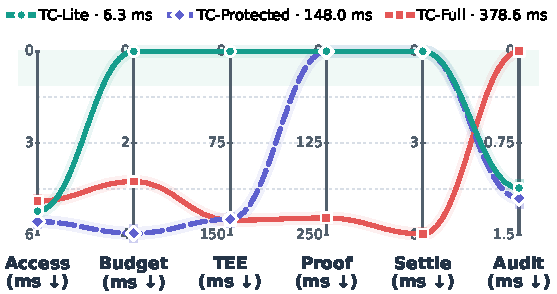
\includegraphics[width=\linewidth]
{Figure/figures/deployment-profiles/deployment_profile_a_latency_reused.pdf}
\caption{Lifecycle latency profile.}
\label{fig:deployment_profile_latency}
\end{subfigure}
\hfill
\begin{subfigure}[t]{0.48\textwidth}
\centering
\includegraphics[width=\linewidth]
{Figure/figures/deployment-profiles/deployment_profile_b_cost_resource_reused.pdf}
\caption{Deployment cost--resource profile.}
\label{fig:deployment_profile_cost_resource}
\end{subfigure}

\caption{Retained component-profile cost and assurance trade-offs. Independent axis scales place the preferable direction upward; hollow N/A markers denote stages absent from a profile rather than zero-cost execution. TC-Lite excludes CP-ABE/AES payload work; TC-Protected adds prepared trusted-processing and privacy-accounting components; TC-Full adds the legacy proof stage. These profiles predate the canonical VCP measurement.}
\label{fig:deployment_profiles}
\end{figure*}

\subsection{Component Costs and Cryptographic Scaling}
\label{subsec:cost_breakdown}

We separate three measurement boundaries: component-level EVM state transitions, compliance-proof generation and verification, and off-chain privacy and encryption costs. Figure~\ref{fig:deployment_profiles} reports retained component profiles, Table~\ref{tab:onchain_lifecycle_cost} reports individual lifecycle operations without the exported verifier, and Table~\ref{tab:zk_compliance_cost} reports the canonical Groth16 VCP boundary. These workloads should not be added or interpreted as interchangeable end-to-end totals.

\subsubsection{Lifecycle EVM State Costs}

Table~\ref{tab:onchain_lifecycle_cost} separates asset-initialization calls from the operations exercised by one request lifecycle. The initialization calls, \texttt{registerAsset} and \texttt{registerBudget}, sum to $209{,}388$ gas when each is executed once. The listed request-path operations sum to $428{,}648$ gas before the exported verifier call. These sums are descriptive aggregates of component means rather than complete \textsf{TC-Full} transaction costs.

The largest component costs arise from \texttt{registerAsset}, \texttt{requestAccess}, and \texttt{reserveBudget}, which create or modify durable contract state. In contrast, proof-metadata submission, audit recording, request approval, and completion each require approximately $25$K--$31$K gas.

\begin{table}[!t]
\centering
\caption{Component-level lifecycle gas excluding the exported proof verifier. Asset initialization is separated from the request-specific lifecycle. Each operation is measured over 120 Hardhat executions.}
\label{tab:onchain_lifecycle_cost}
\begin{tabular}{@{}lrr@{}}
\toprule
\textbf{Operation} & \textbf{Mean gas} & \textbf{Std.} \\
\midrule
\multicolumn{3}{@{}l}{\textit{Asset initialization}} \\
\texttt{registerAsset}             & 136{,}820 & 7.6 \\
\texttt{registerBudget}            & 72{,}568  & 4.7 \\
\midrule
\multicolumn{3}{@{}l}{\textit{Request lifecycle}} \\
\texttt{requestAccess}             & 136{,}679 & 6.3 \\
\texttt{approveRequest}            & 30{,}899  & 4.5 \\
\texttt{reserveBudget}             & 120{,}497 & 6.3 \\
\texttt{submitProof} (metadata)    & 25{,}338  & 17.0 \\
\texttt{consumeBudget}             & 58{,}775  & 6.3 \\
\texttt{completeRequest}           & 30{,}927  & 4.5 \\
\texttt{recordAudit}               & 25{,}533  & 7.2 \\
\bottomrule
\end{tabular}
\end{table}

The verifier is excluded because its cost is evaluated independently below. Table~\ref{tab:onchain_lifecycle_cost} is a component benchmark and should not be used to reconstruct the integrated profile in Fig.~\ref{fig:deployment_profiles}: it uses simpler registration and access-request entry points, standalone budget operations, and a mock proof-metadata call. In contrast, the integrated profile uses context-rich registration and request calls, persists the full expectation state, and performs proof verification, nullifier consumption, budget transition, request completion, and audit recording inside the final settlement path. The Base Sepolia experiment in Section~\ref{subsec:public_testnet} measures yet another boundary: one atomic settlement transaction.

\subsubsection{Canonical VCP Cost}

Table~\ref{tab:zk_compliance_cost} reports the canonical $2\times2$ policy-family circuit used by settlement. The benchmark uses two warm-ups followed by $30$ retained proofs. Prove-only time excludes witness generation; the full proving boundary includes both. The $256$-byte ABI value counts only Groth16 $A/B/C$, while the $24$ public signals remain separate verifier arguments.

\begin{table}[!t]
\centering
\caption{Canonical VCP proof costs. Gas denotes the isolated exported-verifier transaction and excludes lifecycle state transitions.}
\label{tab:zk_compliance_cost}
\scriptsize
\resizebox{\columnwidth}{!}{%
\begin{tabular}{@{}lr@{}}
\toprule
\textbf{Metric} & \textbf{Measured value} \\
\midrule
Public/private inputs & $24/12$ \\
R1CS constraints & $40{,}161$ \\
Witness generation, mean & $73.19$ ms \\
Prove-only, mean / p50 / p95 & $1{,}006.86/1{,}006.39/1{,}043.15$ ms \\
Witness plus prove, mean & $1{,}080.05$ ms \\
Off-chain verification, mean & $8.43$ ms \\
Groth16 $A/B/C$ ABI & $256$ B \\
snarkjs proof JSON, p50 (range) & $723$ B ($719$--$725$ B) \\
Proof plus public JSON, p50 (range) & $1{,}761$ B ($1{,}757$--$1{,}763$ B) \\
Proving / verification key & $18{,}922{,}429/7{,}147$ B \\
Isolated verifier gas, p50 / p95 & $374{,}753/374{,}765$ \\
\bottomrule
\end{tabular}%
}
\end{table}

The generated R1CS, verification key, verifier, and benchmark rows are hash-bound in the VCP evidence manifest. A real-proof integration test verifies two distinct policy matrices with the same key, settles both requests atomically, and rejects a mutation of each of the $24$ public fields. This demonstrates setup reuse within the fixed $2\times2$ policy family and request-wide public-input binding; it does not claim reuse across changed circuit dimensions.

The measured path evaluates Poseidon commitments inside $\mathcal{R}_{\mathrm{VCP}}$ and uses Keccak-256 for EVM-native bookkeeping; independent Solidity-level Poseidon recomputation is outside this measurement boundary.

\subsubsection{Privacy Utility and Access-Control Overhead}

The off-chain experiments evaluate privacy utility, CP-ABE policy scaling, symmetric payload processing, and memory growth. The differential-privacy workload contains $50{,}000$ synthetic healthcare records and six bounded aggregate queries: three counts with $\Delta f=1$ and three means with $\Delta f=R/n$, calibrated from CDC NHANES marginals\footnote{\url{https://wwwn.cdc.gov/nchs/nhanes/}}. At $\varepsilon=1.0$, the diabetes-count query has $0.044\%$ relative error, while the mean-query errors remain below $0.012\%$. At $\varepsilon=0.1$, the count-query errors range from $0.40\%$ to $0.47\%$, and the mean-query errors remain between approximately $0.085\%$ and $0.11\%$.

Figure~\ref{fig:abe_policy_scaling} compares the lightweight KEM--DEM baseline with the collusion-resistant AC17/FAME CP-ABE implementation provided by \texttt{rabe} 0.4.2~\cite{agrawal2017fame}. As policy size increases from $5$ to $25$ leaves, full CP-ABE encryption grows from approximately $51$ to $181$ ms, whereas KEM--DEM encryption grows from approximately $6$ to $35$ ms. Full CP-ABE decryption remains near $23$--$24$ ms because the satisfying attribute set is fixed while the total policy expands. The comparison therefore measures the additional cost of the deployed collusion-resistant backend rather than attributing that guarantee to the lightweight baseline.

Because CP-ABE encapsulates only the AES payload key, its cost depends on policy complexity rather than payload length. Figure~\ref{fig:abe_bulk_throughput} shows AES-256-GCM throughput of approximately $1.3$--$1.4$ GB/s. Figure~\ref{fig:abe_memory_footprint} shows near-linear memory growth because the benchmark retains plaintext and ciphertext buffers simultaneously.

\begin{figure}[!t]
\centering
\begin{subfigure}[t]{0.48\columnwidth}
\centering
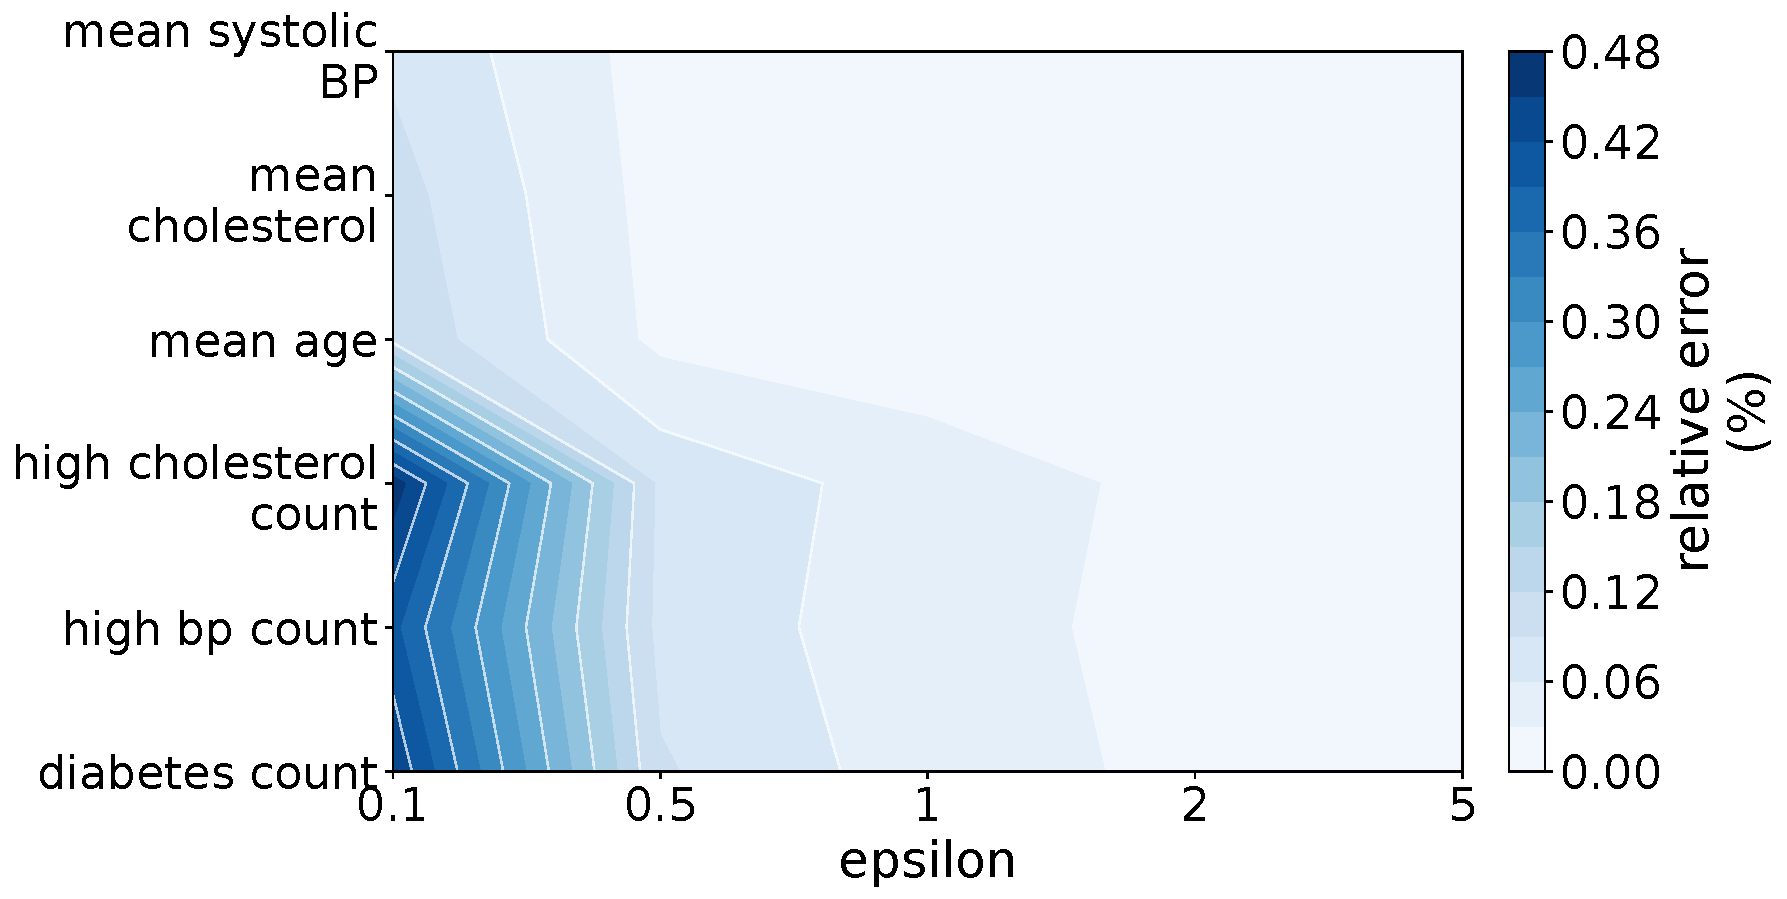
\includegraphics[width=\linewidth]
{Figure/figures/dp/d3_error_contour.pdf}
\caption{DP relative error.}
\label{fig:dp_relative_error}
\end{subfigure}
\hfill
\begin{subfigure}[t]{0.48\columnwidth}
\centering
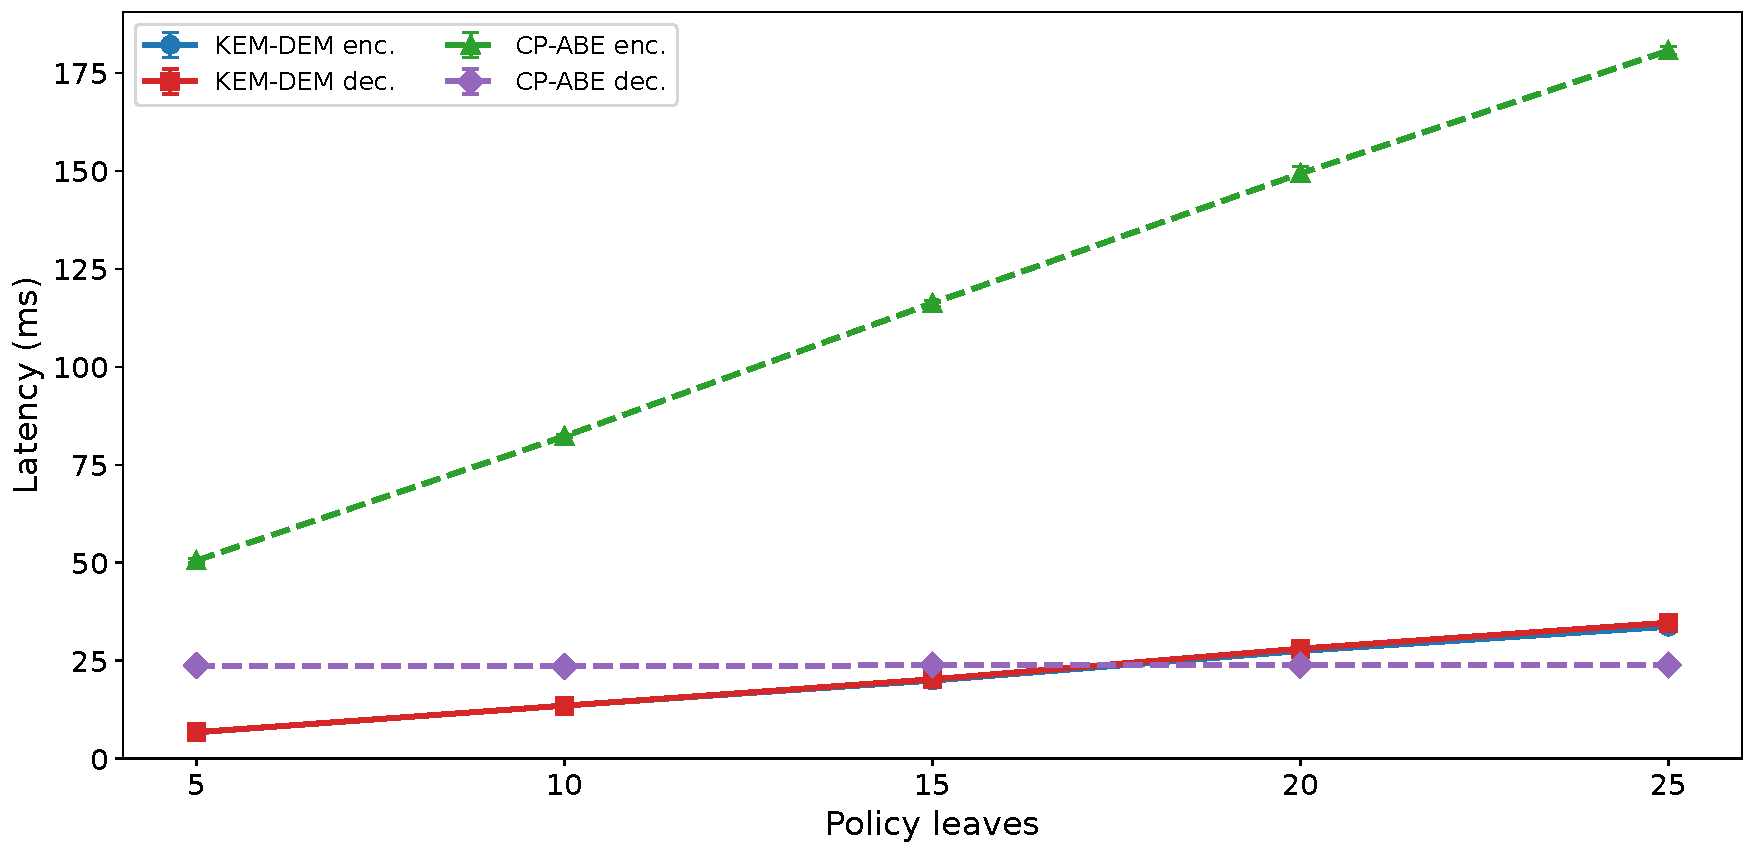
\includegraphics[width=\linewidth]
{Figure/figures/abe/ab1_policy_time_revised.pdf}
\caption{Full CP-ABE and KEM--DEM scaling.}
\label{fig:abe_policy_scaling}
\end{subfigure}

\vspace{0.45em}

\begin{subfigure}[t]{0.48\columnwidth}
\centering
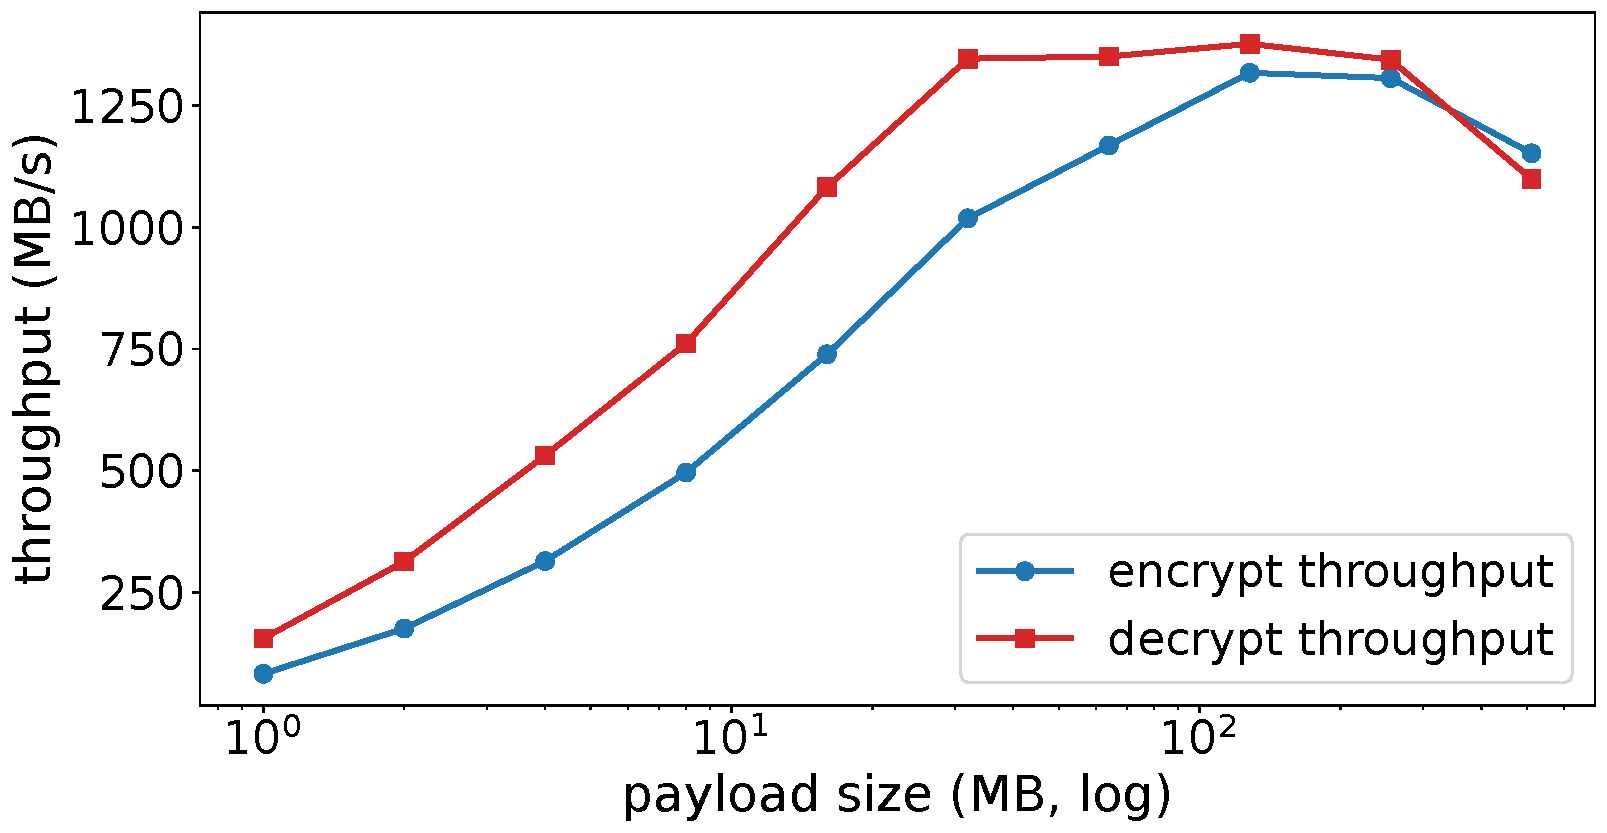
\includegraphics[width=\linewidth]
{Figure/figures/abe/ab4_throughput.pdf}
\caption{AES-GCM throughput.}
\label{fig:abe_bulk_throughput}
\end{subfigure}
\hfill
\begin{subfigure}[t]{0.48\columnwidth}
\centering
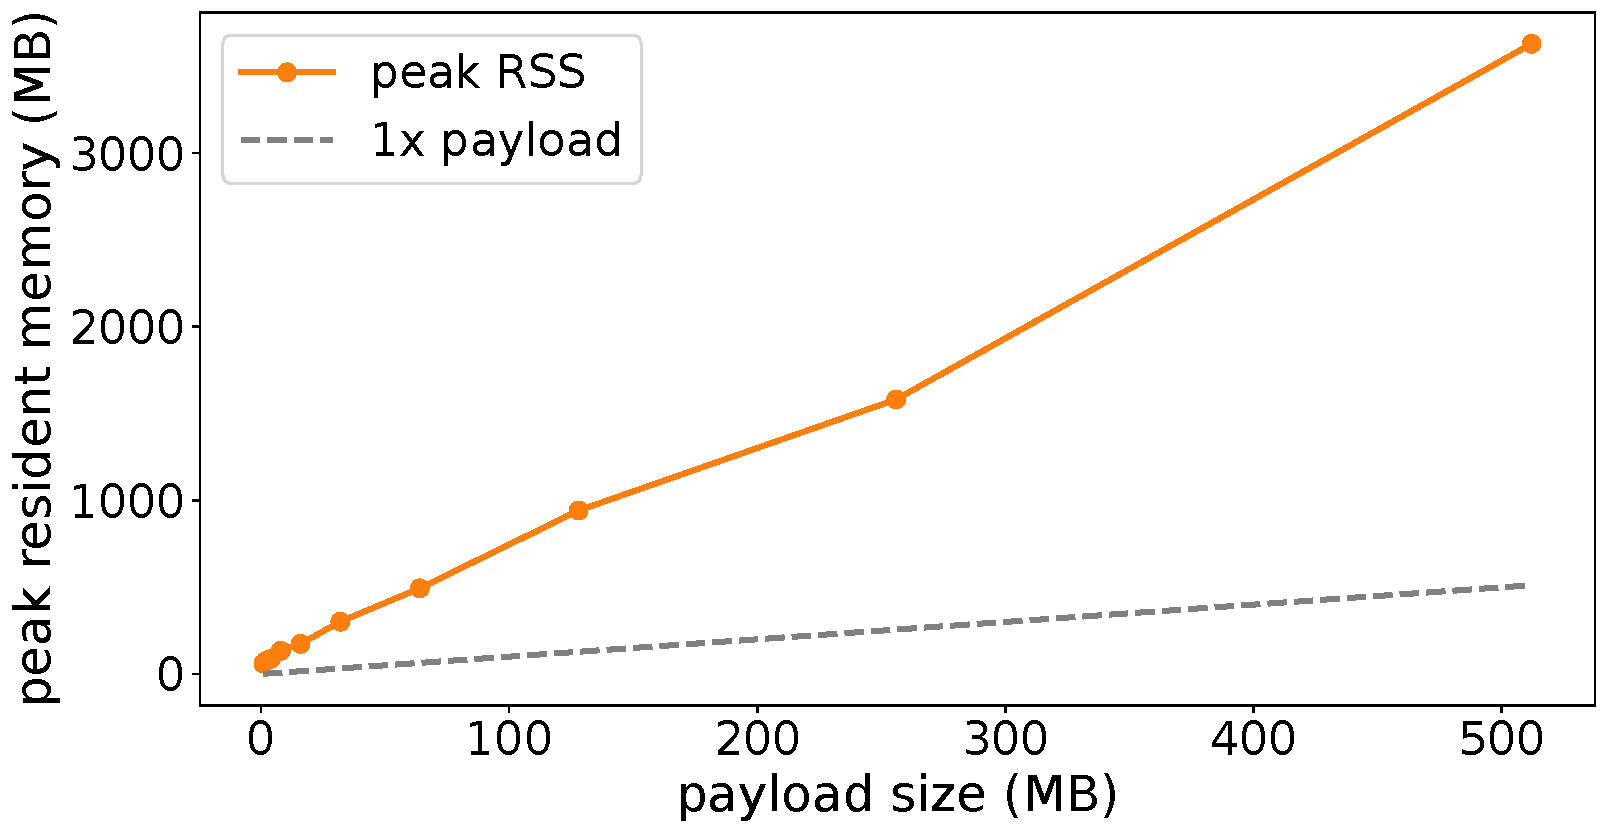
\includegraphics[width=\linewidth]
{Figure/figures/abe/ab6_peak_rss.pdf}
\caption{Peak resident memory.}
\label{fig:abe_memory_footprint}
\end{subfigure}

\caption{Off-chain privacy and access-control costs. Panel (a) reports the privacy--utility trade-off; panel (b) compares the deployed AC17/FAME backend with the KEM--DEM baseline; panels (c) and (d) report symmetric payload throughput and memory growth.}
\label{fig:offchain_privacy_access}
\end{figure}

Overall, the results separate asset initialization, recurring lifecycle state, proof generation and verification, and bulk-data protection into explicit measurement boundaries. Persistent state updates and prover-side compliance generation account for the principal costs, while CP-ABE overhead remains policy-dependent and bulk payload processing remains dominated by symmetric encryption.
\subsection{Trusted-Processor Scalability and Policy-Level Deviation Analysis}
\label{subsec:tee_scaling_robustness}

\begin{figure*}[!t]
\centering

\begin{subfigure}[t]{0.32\textwidth}
\centering
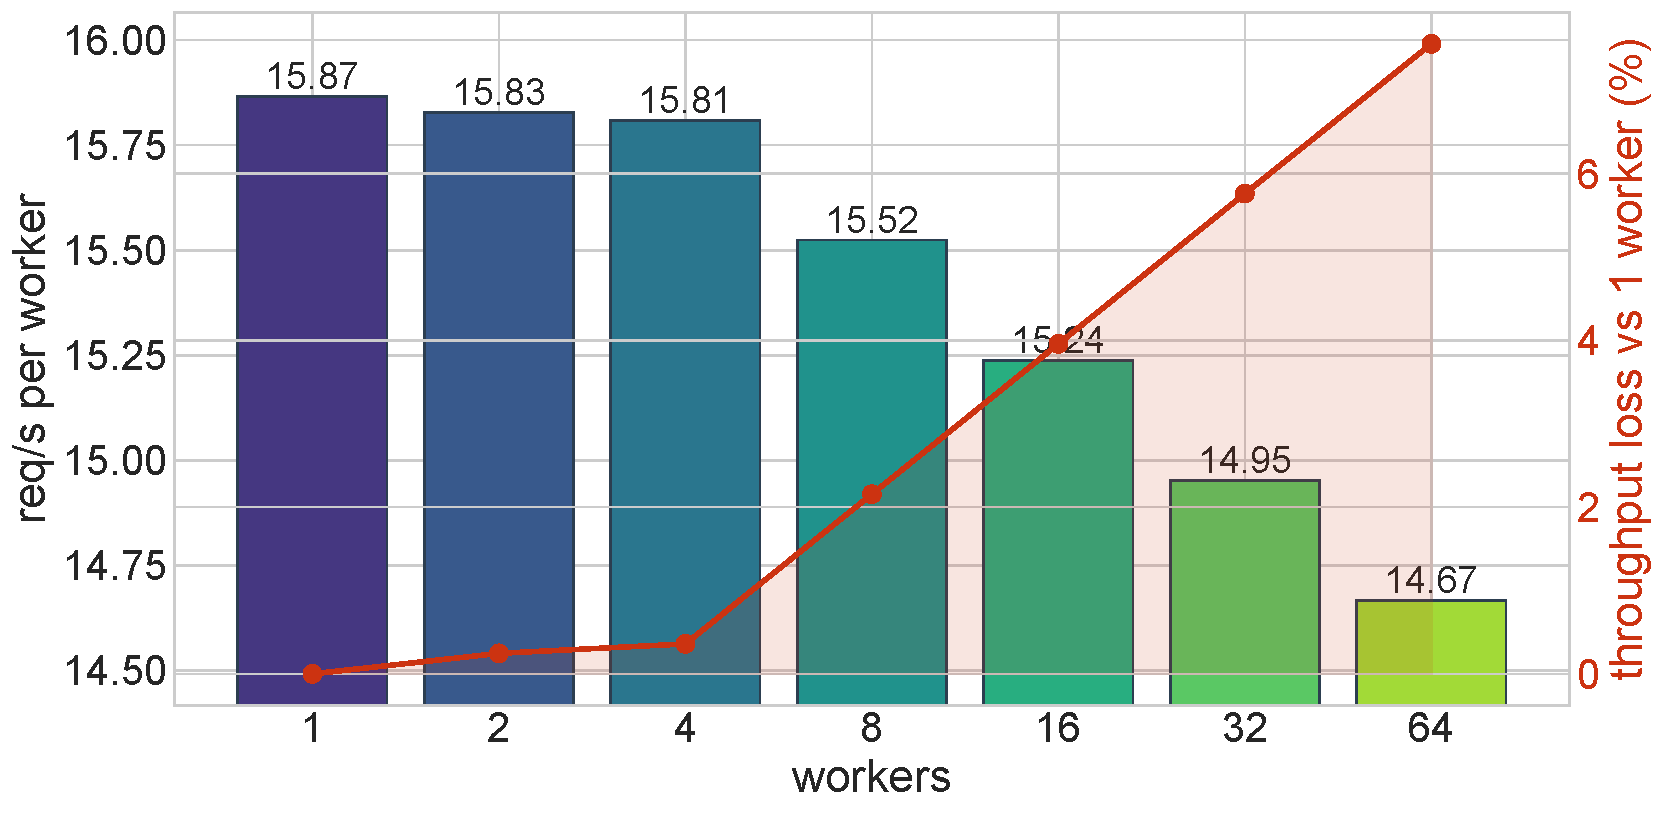
\includegraphics[width=\linewidth]
{Figure/figures/nitro_new/nitro_pool_per_worker_throughput.pdf}
\caption{Per-worker throughput.}
\label{fig:nitro_per_worker_throughput}
\end{subfigure}
\hfill
\begin{subfigure}[t]{0.32\textwidth}
\centering
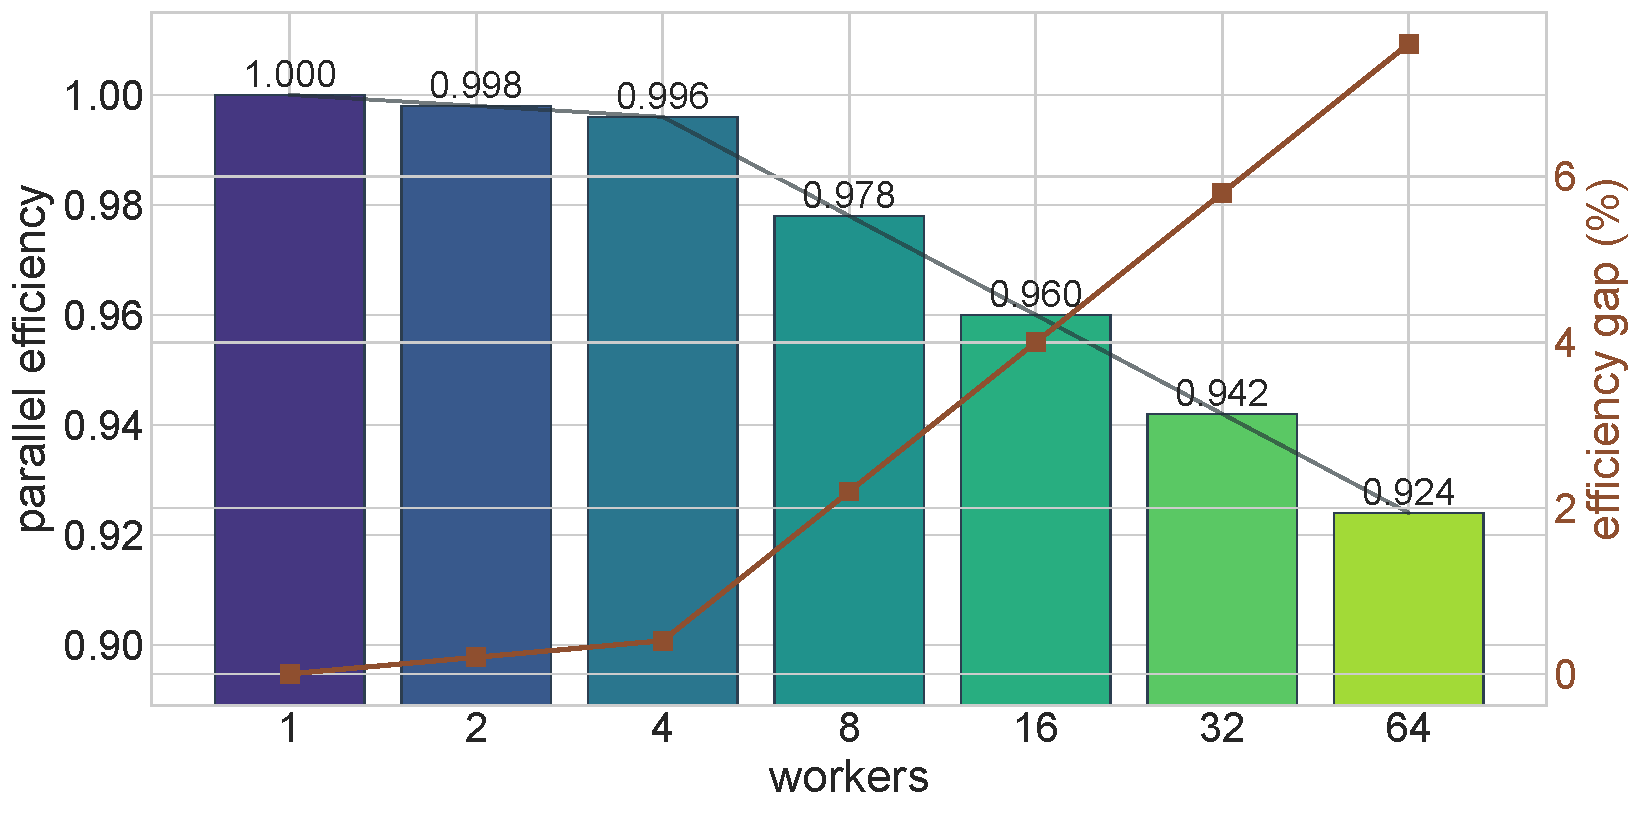
\includegraphics[width=\linewidth]
{Figure/figures/nitro_new/nitro_pool_parallel_efficiency.pdf}
\caption{Parallel efficiency.}
\label{fig:nitro_parallel_efficiency}
\end{subfigure}
\hfill
\begin{subfigure}[t]{0.32\textwidth}
\centering
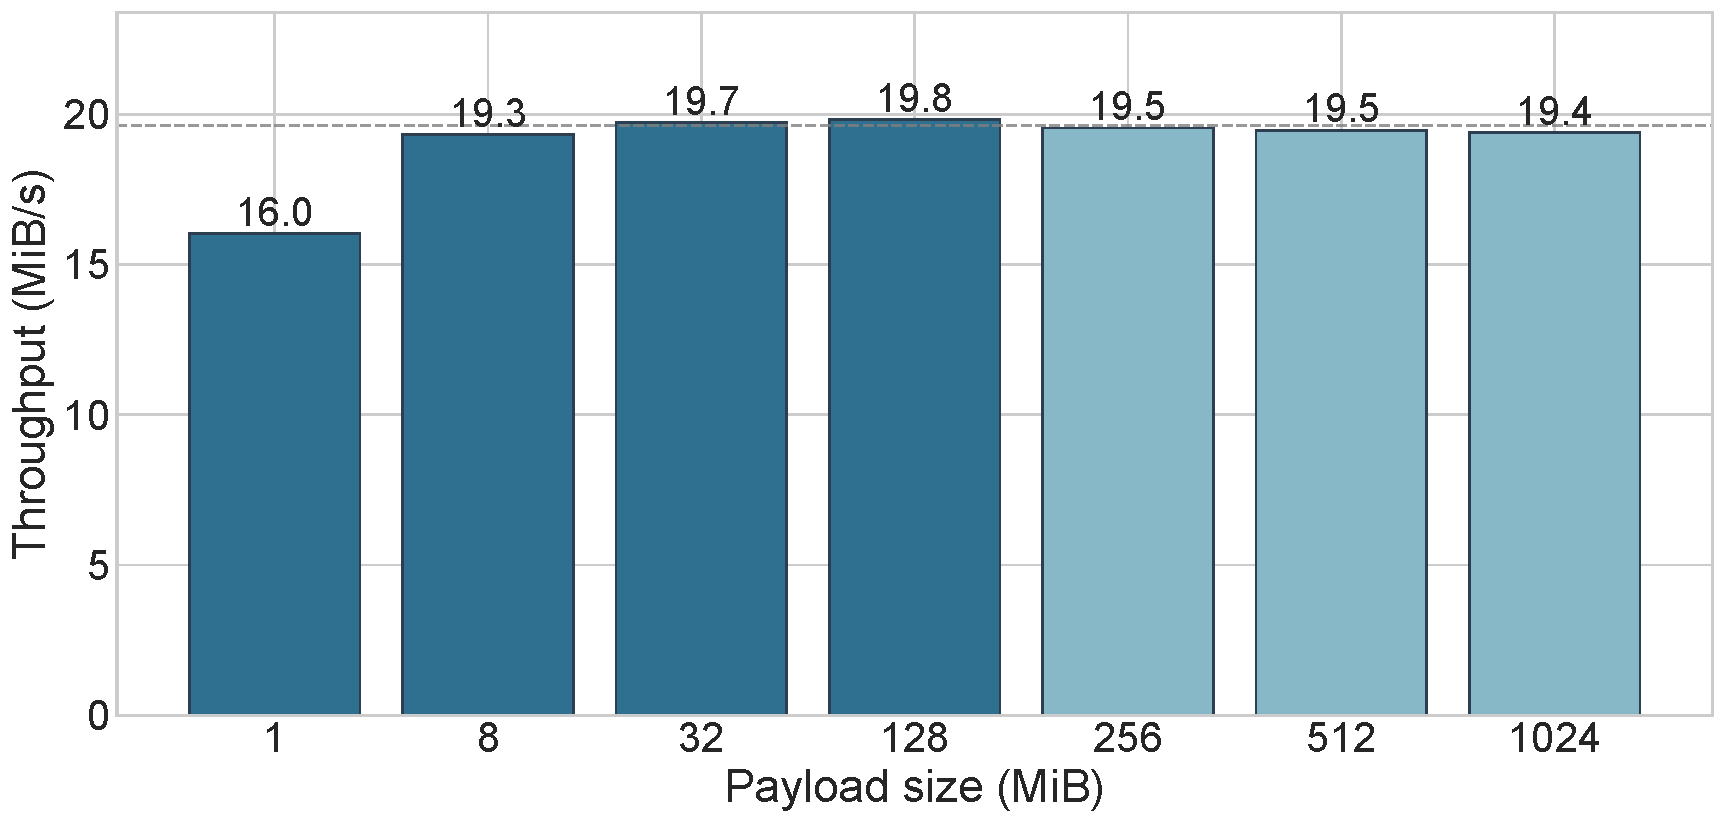
\includegraphics[width=\linewidth]
{Figure/figures/nitro_new/nitro_payload_throughput.pdf}
\caption{Payload throughput.}
\label{fig:nitro_payload_throughput}
\end{subfigure}

\vspace{0.35em}

\begin{subfigure}[t]{0.32\textwidth}
\centering
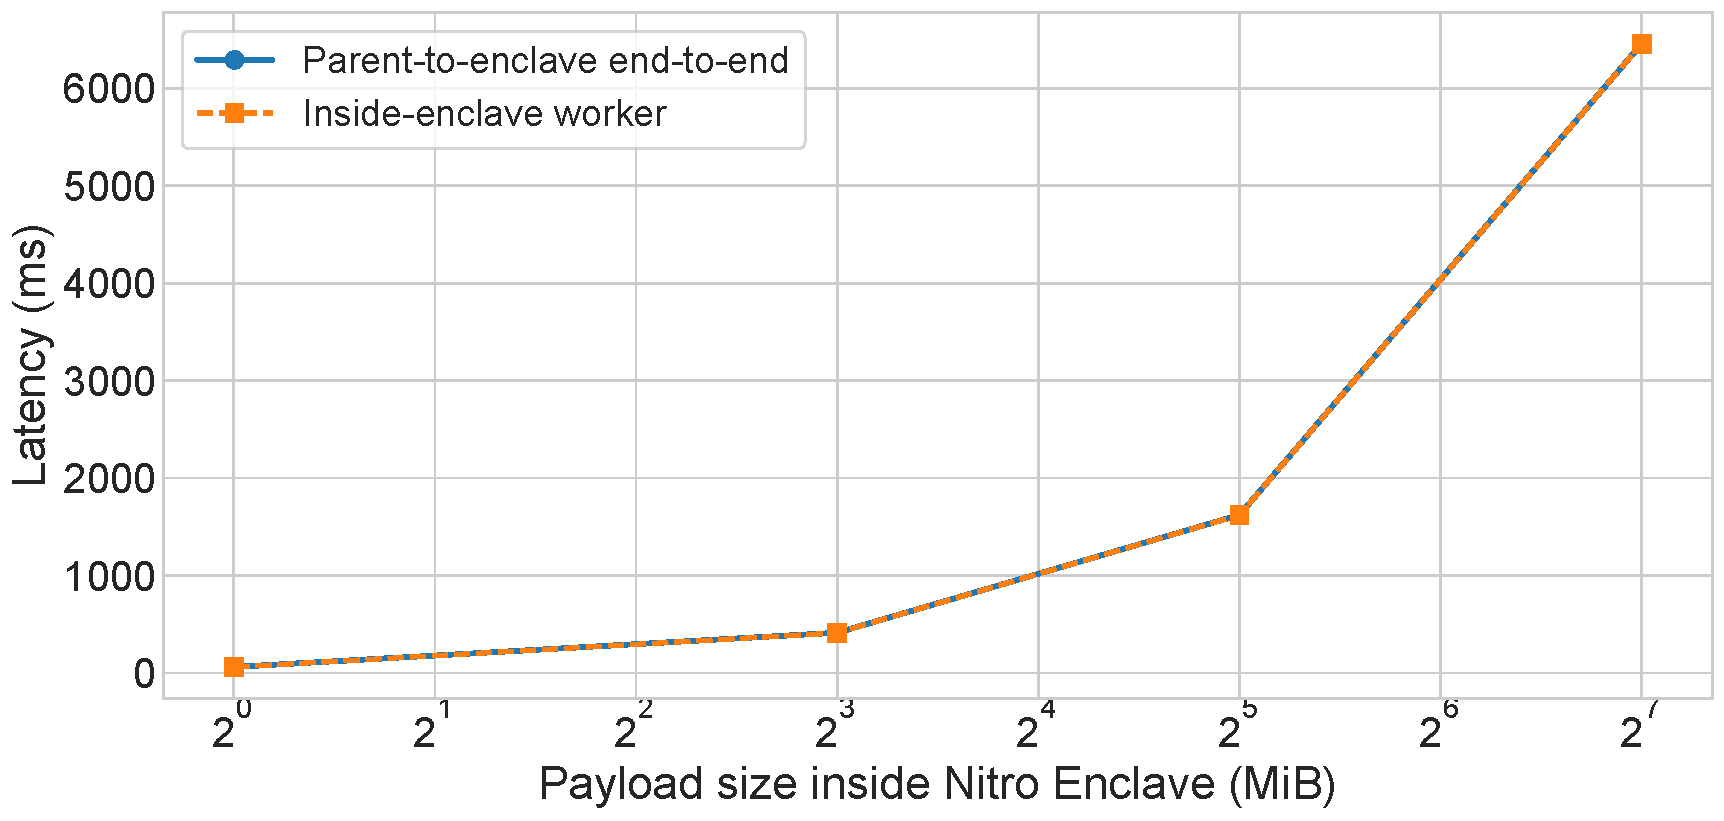
\includegraphics[width=\linewidth]
{Figure/figures/nitro_new/nitro_latency_vs_payload.pdf}
\caption{Payload-dependent latency.}
\label{fig:nitro_latency_vs_payload}
\end{subfigure}
\hfill
\begin{subfigure}[t]{0.32\textwidth}
\centering
\includegraphics[width=\linewidth]
{Figure/figures/tee_robustness/r2_subtle_detection.pdf}
\caption{Deviation-detection rate.}
\label{fig:tee_detection_severity}
\end{subfigure}
\hfill
\begin{subfigure}[t]{0.32\textwidth}
\centering
\includegraphics[width=\linewidth]
{Figure/figures/tee_robustness/r3_attack_success.pdf}
\caption{Deviation-evasion rate.}
\label{fig:tee_evasion_severity}
\end{subfigure}

\caption{Trusted-processor scaling and policy-level deviation analysis. Panels (a)--(b) report worker-pool projections calibrated from the measured Nitro configuration; panels (c)--(d) report measured payload behavior inside the Nitro data path; and panels (e)--(f) quantify the response of protocol-level deviation detectors. The latter results do not constitute a hardware side-channel or platform-compromise evaluation.}
\label{fig:trusted_processor_scalability_robustness}
\end{figure*}

The trusted-processor evaluation separates measured Nitro execution, model-based pool scaling, and protocol-level deviation analysis. The Nitro configuration uses EIF-based workers, fixed enclave resources, and a VSOCK parent--enclave channel, as reported in Table~\ref{tab:experiment_setup}. Worker counts beyond the directly measured configuration are projections calibrated from the measured service rate and contention behavior; they are not presented as a 64-enclave physical deployment.

Let $X_w$ denote aggregate throughput with $w$ workers. Per-worker
throughput and parallel efficiency are defined as
\begin{equation}
\begin{aligned}
x_w
&=
\frac{X_w}{w},
\\
E_w
&=
\frac{X_w}{wX_1}.
\end{aligned}
\label{eq:pool_scaling_metrics}
\end{equation}
Fig.~\ref{fig:nitro_per_worker_throughput} shows that $x_w$ remains
close to the single-worker rate at moderate pool sizes and then
decreases gradually as shared host resources become saturated.
The corresponding $E_w$ curve in
Fig.~\ref{fig:nitro_parallel_efficiency} remains near unity initially,
but its marginal gain declines as scheduling, memory pressure, VSOCK
communication, and orchestration costs accumulate. The absence of a
sharp collapse indicates gradual host-level saturation rather than a
discrete enclave-memory threshold.

Payload experiments expose a different bottleneck. Fig.~\ref{fig:nitro_payload_throughput} shows that the steady-state data rate stabilizes for medium and large payloads, whereas Fig.~\ref{fig:nitro_latency_vs_payload} shows increasing request latency as the encrypted working set grows. The growth is decomposed in Fig.~\ref{fig:nitro_latency_composition}, where transfer, transcript hashing, enclave computation, response handling, and native attestation contribute additively to the critical path. These results indicate that large TrustCircuit assets should be streamed, partitioned, or processed in bounded batches rather than materialized as unrestricted enclave buffers.

\begin{figure}[!t]
\centering

\begin{subfigure}[t]{0.95\columnwidth}
\centering
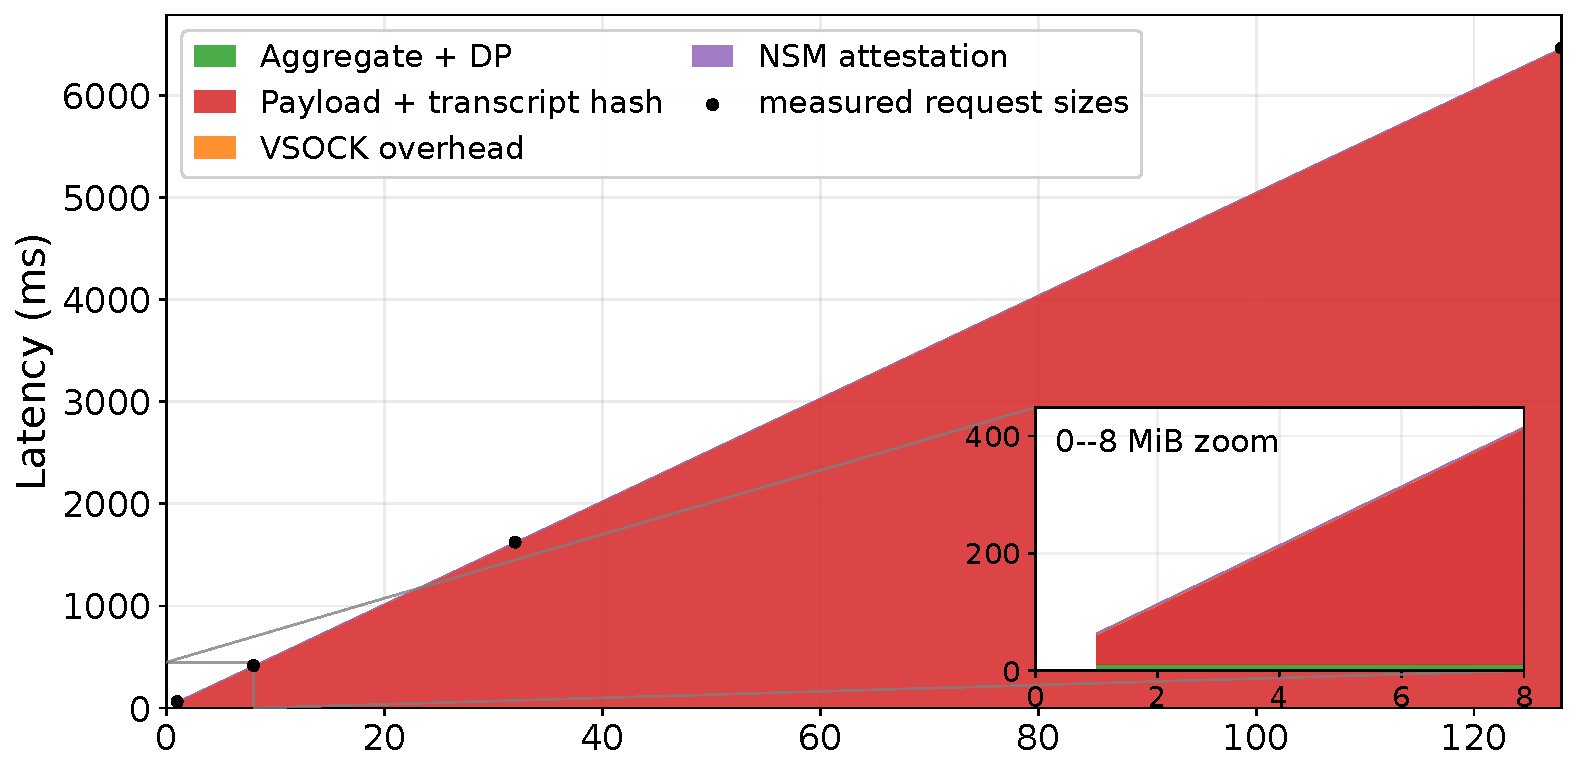
\includegraphics[width=\linewidth]
{Figure/figures/nitro_new/n1_latency_composition_area.pdf}
\caption{Latency composition under encrypted working-set growth.}
\label{fig:nitro_latency_composition}
\end{subfigure}

\vspace{0.35em}

\begin{subfigure}[t]{0.95\columnwidth}
\centering
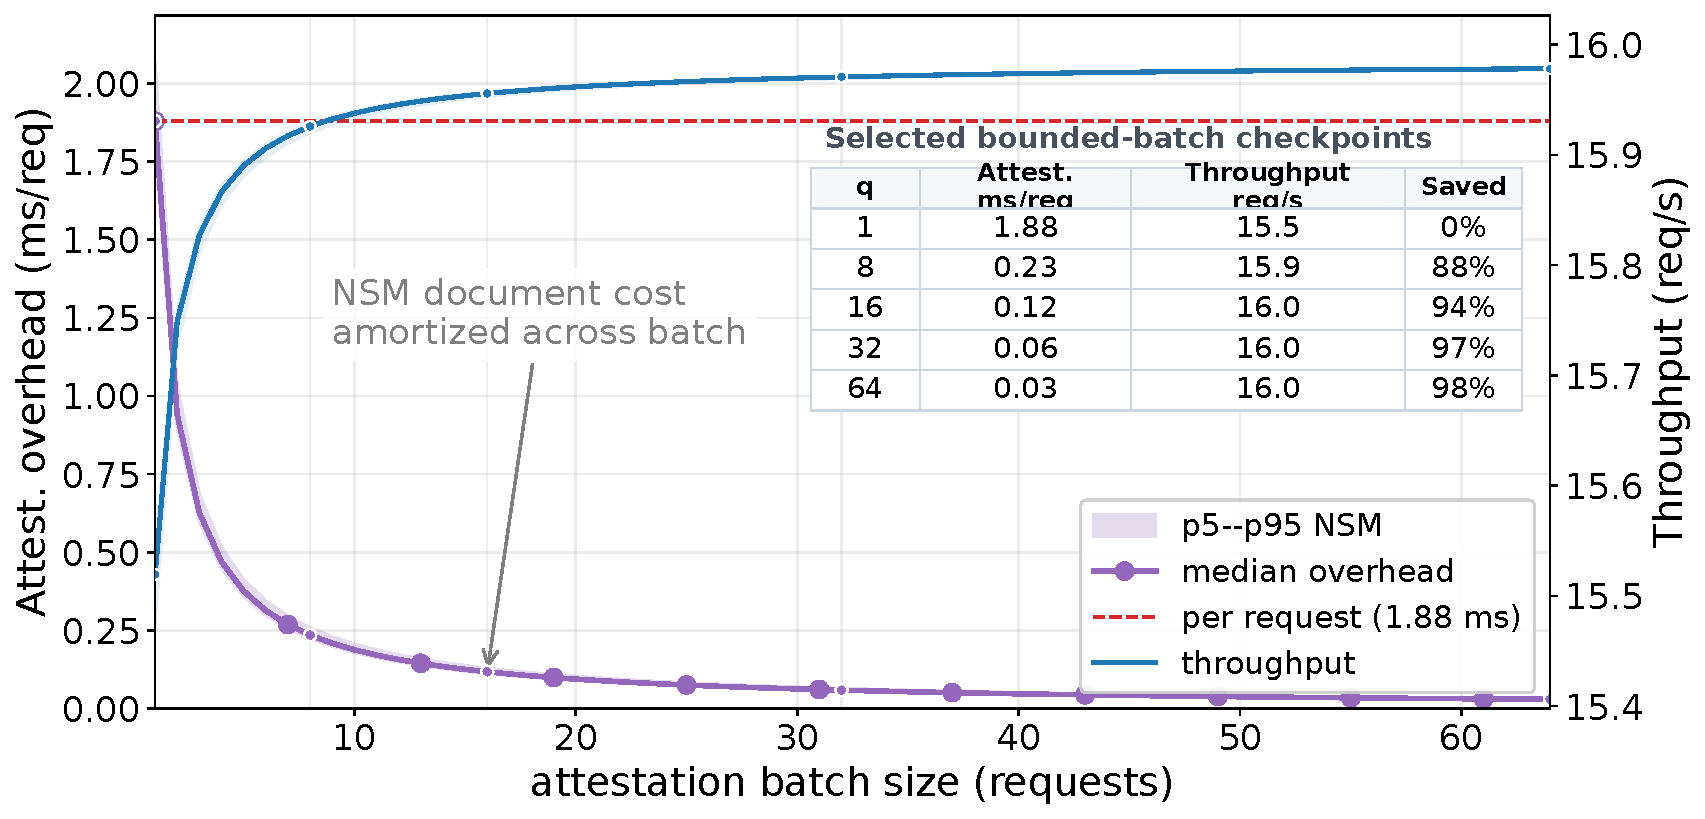
\includegraphics[width=\linewidth]
{Figure/figures/nitro_new/n3_attestation_amortization.pdf}
\caption{Attestation overhead under request batching.}
\label{fig:nitro_attestation_amortization}
\end{subfigure}

\caption{Measured-parameter projections for the Nitro trusted-processor path. Panel (a) decomposes request latency as the encrypted working set grows. Panel (b) shows how reusing one validated attestation statement across a bounded batch reduces fixed per-request attestation overhead.}
\label{fig:nitro_model_projection}
\end{figure}

Fig.~\ref{fig:nitro_attestation_amortization} isolates the fixed cost of native attestation. Without batching, every request independently pays the document-generation and validation cost. For a batch of $q$ requests covered by one bounded attestation context, the amortized component is approximately $T_{\mathrm{att}}/q$. Batching therefore recovers part of the throughput otherwise lost to repeated attestation, provided that every request remains individually bound through its request identifier, result commitment, privacy expenditure, and nullifier.

Robustness analysis distinguishes deterministic rejection from statistical deviation detection. Invalid purposes, disallowed functions, stale policy versions, budget violations, replayed nullifiers, commitment mismatches, and invalid validated-attestation statements fail explicit protocol predicates. Their rejection does not depend on a statistical detector.

The detector is used only for outputs that remain syntactically well-formed but deviate from the expected release behavior, including result perturbation, privacy-cost misreporting, attestation-field deviation, and omitted or weakened DP noise. For deviation class $a$ and severity $s$, let $N_{a,s}$ be the number of injected cases and $N_{a,s}^{\mathrm{det}}$ the number detected. We report
\begin{equation}
\begin{aligned}
\mathrm{DR}_{a}(s)
&=
\frac{N_{a,s}^{\mathrm{det}}}{N_{a,s}},
\\
\mathrm{ER}_{a}(s)
&=
1-\mathrm{DR}_{a}(s).
\end{aligned}
\label{eq:deviation_detection_metrics}
\end{equation}
Figs.~\ref{fig:tee_detection_severity} and \ref{fig:tee_evasion_severity} show monotonic separation as the injected deviation becomes larger: detection increases and evasion decreases. At low severity, the modified releases remain closer to the expected output distribution and are correspondingly harder to distinguish.

These results characterize the sensitivity of secondary protocol-level checks around the trusted-processor workflow. They do not prove correctness of the DP random sampler, and they do not extend VCP into a proof of arbitrary enclave computation. Side channels, compromised attestation roots, malicious approved code, rollback within an untrusted execution platform, and common-mode TEE compromise remain governed by the assumptions formalized in Section~\ref{sec:security}.

\subsection{Public Testnet Deployment and Settlement}
\label{subsec:public_testnet}

We deployed the final eight-contract VCP suite once on Base Sepolia, chain ID 84532, and submitted $30$ valid request lifecycles containing real $24$-input Groth16 proofs. The campaign comprises $135$ successful transactions and ends with exactly $12{,}000{,}000$ fixed-point budget units consumed ($30\times400{,}000$). Public-testnet measurements cover deployment, valid settlement, total transaction fee, and one-confirmation inclusion. Context substitution, tampered inputs, invalid proofs, and replay rejection are evaluated separately by the local real-proof and contract test suites rather than attributed to this public campaign.

\begin{figure*}[!t]
\centering

\begin{subfigure}[t]{0.47\textwidth}
\centering
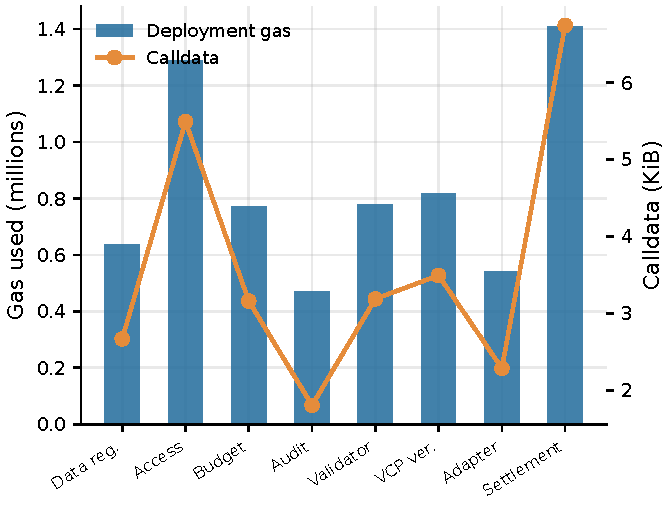
\includegraphics[width=\linewidth]{Figure/figures/base-sepolia/figure_1a_deployment_resources.pdf}
\caption{Contract deployment resources.}
\label{fig:testnet_deployment_resources}
\end{subfigure}
\hfill
\begin{subfigure}[t]{0.47\textwidth}
\centering
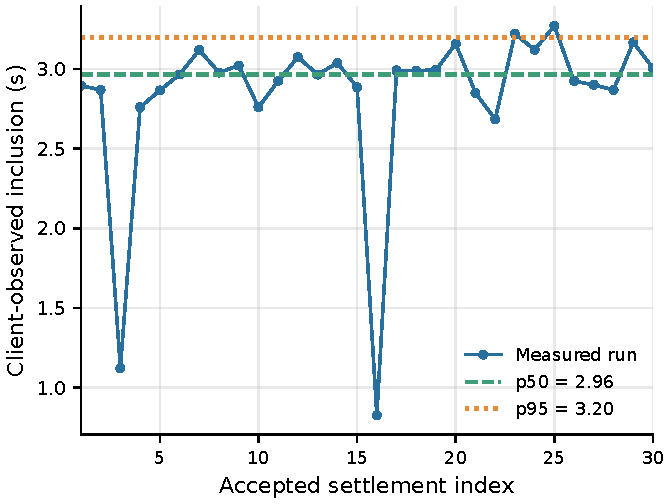
\includegraphics[width=\linewidth]{Figure/figures/base-sepolia/figure_2a_settlement_latency.pdf}
\caption{One-confirmation inclusion latency.}
\label{fig:testnet_settlement_latency}
\end{subfigure}

\caption{Final-stack TrustCircuit evaluation on Base Sepolia. Panel (a) reports one-time deployment gas and calldata for all eight contracts. Panel (b) reports client-observed one-confirmation latency for $30$ accepted real-proof settlements.}
\label{fig:base_sepolia_evaluation}
\end{figure*}

Figure~\ref{fig:testnet_deployment_resources} shows that deploying the eight-contract suite requires $6{,}714{,}037$ gas and $29{,}517$ bytes of deployment calldata. Individual costs range from $471{,}981$ gas for the audit ledger to $1{,}409{,}823$ gas for the settlement contract. The added validator registry and canonical VCP verifier are included in this total. These costs are incurred once and amortized across subsequent requests.

The campaign used a fixed $6{,}000{,}000$-wei gas price. A valid settlement costs $3.326976~\mu\mathrm{ETH}$ at the median and $3.327258~\mu\mathrm{ETH}$ at the 95th percentile. Because testnet ETH has no market value, these values are reproducible fee observations rather than USD or mainnet cost forecasts.

Figure~\ref{fig:testnet_settlement_latency} shows that valid settlement reaches one-confirmation inclusion in $2.964$ seconds at the median and $3.196$ seconds at the 95th percentile. Proofs are prepared and verified off-chain before transaction submission, so these values measure broadcast-to-inclusion rather than proof generation. The campaign demonstrates that request validation, Groth16 verification, nullifier consumption, budget consumption, completion, and audit recording execute successfully within one public-testnet transaction.

\subsection{Comparison With Counterparts}
\label{subsec:cross_system_enforcement}

We compare TrustCircuit with representative systems only at the closest recurring operation reported in each original evaluation: proof generation, trusted execution, or ledger-backed verification. These boundaries differ in statement scope, hardware, serialization, and deployment environment; the comparisons provide scale, not interchangeable end-to-end rankings.

\textit{Comparison with VLDP:} VLDP attaches a non-interactive proof to each locally randomized report~\cite{bontekoe2024efficient}. Its Base, Expand, and Shuffle configurations require $55{,}884$--$174{,}095$ constraints and $0.610$--$1.821$~s for the proof-bearing client step. VCP uses $40{,}161$ constraints, $28.1\%$--$76.9\%$ fewer than that reported range, while its $1.007$-s mean prove-only time lies within VLDP's published latency range. The systems prove different relations, so this is not a universal prover-speed claim.

\textit{Comparison with VerifBFL:} VerifBFL reports $2.189$~s and a $35.4$~KB proof for aggregation of five local models~\cite{bellachia2025verifbfl}. Against those published values, VCP's $1.007$-s prove-only mean is approximately $2.17\times$ faster, and its $723$-byte median snarkjs proof JSON is approximately $49\times$ smaller. VCP instead proves a request-lifecycle relation and binds the accepted proof to the current request, reserved budget, execution context, nullifier, and audit transition; the ratios therefore compare serialization and proving boundaries, not identical statements.

\textit{Comparison with Veracruz:} Veracruz reports approximately $2.7$~s of fixed Nitro initialization~\cite{brossard2023private}. TrustCircuit likewise separates provisioning from recurring work. The retained measured/composed legacy \textsf{TC-Full} profile is $378.6$~ms, while the canonical VCP prove-only boundary is $1.007$~s. Native attestation generation contributes a median $1.88$~ms in the retained Nitro experiment. These are component boundaries rather than one continuous final-stack trace.

\textit{Comparison with ProMark and VPrivKV:} ProMark generates campaign tokens in $0.01$--$0.05$~s but defers campaign-wide verification, which requires $66.39$--$501.96$~min in its largest reported workloads~\cite{hoang2024promark}. TrustCircuit instead settles every accepted data-use request individually. On Base Sepolia, one final-stack atomic settlement performs context checking, proof verification, nullifier consumption, budget consumption, completion, and audit recording for $554{,}496$ gas at the median, with $2.964$~s median inclusion. VPrivKV verifies sampling and perturbation for individual key--value reports~\cite{zhou2025vprivkv}; TrustCircuit's implemented boundary instead focuses on request-bound ledger state and replay-safe settlement across repeated requests.

The comparison places VCP within VLDP's reported prover-time range and below the cited VerifBFL aggregation boundary, while adding request-level settlement that neither isolated proof generation nor deferred campaign verification captures.
\section{Limitations}
\label{sec:discussion}

TrustCircuit should be interpreted as a prototype-backed framework rather than a production-ready deployment. The evaluation combines controlled Hardhat measurements, AWS Nitro Enclave experiments, and a public Base Sepolia deployment. Hardhat isolates opcode-level gas demand, verifier behavior, rejection conditions, and contract-state transitions, while the final-stack Base Sepolia campaign validates public deployment, real-proof settlement, total fees, and one-confirmation latency for $30$ accepted requests. It does not repeat adversarial reverts on the public chain. The campaign is also limited in duration, workload intensity, and network diversity; it does not characterize sustained congestion, sequencer outages, mainnet fee volatility, adversarial mempool conditions, or production data-availability costs across different Layer-2 systems.

The default settlement path does not recompute general Poseidon commitments in Solidity. Poseidon is evaluated inside the SNARK relation and checked through the exported verifier, whereas Keccak-256 is used for EVM-native storage keys, identifiers, and events. A deployment that introduces Solidity-level Poseidon recomputation, a different verifier implementation, or additional on-chain commitment checks would create a separate gas boundary and must be benchmarked independently.

The trusted-processor results are also limited to the evaluated Nitro configuration. Payload handling, VSOCK communication, enclave execution, and native-attestation overhead are directly measured, whereas the largest worker-pool configurations are model-based projections calibrated from the measured service rate and contention behavior. The attestation-batching results quantify potential amortization of a fixed validation cost, but do not by themselves constitute a complete multi-request attestation protocol. The robustness experiments evaluate protocol-level rejection and statistical deviation detection; they do not establish resistance to side channels, rollback attacks, compromised trust roots, malicious approved code, correlated platform compromise, or operational misconfiguration.

Finally, the privacy and compliance guarantees apply only to the mechanisms and predicates explicitly instantiated by the prototype. The differential-privacy evaluation uses bounded aggregate queries over synthetic data and should not be generalized to arbitrary datasets, streaming workloads, machine-learning training, or interactive analytics. The reference experiment maintains cumulative per-order RDP state, but the current enclave request path does not persist that vector across accepted releases; the paper therefore treats cumulative RDP charging as a protocol/accountant boundary rather than a completed enclave-internal state machine. VCP proves consistency of the encoded policy, budget, result, attestation-context commitment, nullifier, and audit relations. It does not directly validate native TEE certificate chains, prove arbitrary off-chain program correctness, verify the internal differential-privacy sampling procedure, or guarantee legal compliance for rules that have not been correctly translated into the encoded policy. Future work should therefore evaluate longer-running production-oriented Layer-2 deployments, directly measured multi-host trusted-processor pools, explicit batch-attestation constructions, richer compliance relations, and stronger validator and TEE operational hardening.

\section{Conclusion}
\label{sec:conclusion}

TrustCircuit introduces a request-specific lifecycle for accountable privacy-preserving data circulation, binding authorization, privacy-budget reservation and consumption, validated execution context, result commitment, replay-prevention nullifier, proof verification, and audit settlement to the same asset, consumer, request, and policy version. The protocol contributes a conservative fixed-point interface for off-chain R\'enyi accounting, a canonical attestation bridge, and a policy-parameterized VCP relation reusable across a bounded policy family. For the canonical two-rule VCP, Groth16 proves in $1.007$~s on average, emits a $256$-byte A/B/C ABI object ($723$-byte median snarkjs JSON), and requires $374{,}753$ gas at the median for isolated verification. On Base Sepolia, $30$ atomic request-bound settlements through the final eight-contract stack consume $554{,}496$ gas at the median and reach inclusion in $2.964$~s. These results show that request-level policy, privacy, execution, replay, and audit constraints can be coordinated within a practical public Layer-2 settlement path. VCP proves consistency of the encoded request lifecycle; it does not prove arbitrary off-chain computation correctness, internal differential-privacy sampling correctness, native attestation validity, or legal compliance.

Future work will extend TrustCircuit toward production-oriented and more heterogeneous deployments. We plan to evaluate the protocol across additional deployment models, privacy workloads, proof configurations, policy structures, and trusted-execution platforms, including directly measured multi-host processor pools and at least one non-Nitro TEE. Further work will investigate threshold attestation validators, auditable native-evidence retention, validator key rotation and compromise recovery, CP-ABE revocation and ciphertext re-wrapping, explicit batch-attestation protocols, invalid-proof mitigation, and longer-running Layer-2 experiments under varied fee and congestion conditions. These extensions will test the portability, scalability, and operational resilience of the request-indexed lifecycle beyond the current prototype.

\section*{Acknowledgment}
This research is funded by Vietnam National University Ho Chi Minh City (VNU-HCM) under grant number NCM2025-26-01.

% \bibliographystyle{IEEEtran}
% \bibliography{refs}

\bibliographystyle{IEEEtran}
\let\oldthebibliography\thebibliography
\renewcommand{\thebibliography}[1]{\oldthebibliography{#1}\scriptsize\setlength{\itemsep}{0pt}\linespread{0.7}\selectfont}
\bibliography{refs}

\begin{IEEEbiography}
[{\includegraphics[width=1in,height=1.25in,clip,keepaspectratio]{Author/bao.jpg}}]{Bao Huynh:} A third-year undergraduate student pursuing a Bachelor of Engineering in Information Security at the University of Information Technology (UIT), Vietnam National University Ho Chi Minh City (VNU-HCM). His research interests span blockchain systems, network security, and artificial intelligence, with a growing focus on machine learning applications in decentralized environments. He actively explores these domains through academic projects and independent research.
\end{IEEEbiography}

\begin{IEEEbiography}
[{\includegraphics[width=1in,height=1.25in,clip,keepaspectratio]{Author/dung.png}}]{Tuan-Dung Tran:} obtained his Bachelor of Science (2013) and Master of Science (2016) degrees in Computer Science from Ho Chi Minh City University of Science (HCMUS), a constituent institution of Vietnam National University Ho Chi Minh City (VNU-HCM). He is currently pursuing doctoral research in Information Technology at the University of Information Technology (UIT), VNU-HCM. Concurrently, he holds a lectureship within the Department of Information Security, Faculty of Computer Networks \& Communication at UIT. His principal research interests encompass security and privacy, blockchain and distributed systems, machine learning, artificial intelligence, and federated learning.
\end{IEEEbiography}

\begin{IEEEbiography}
[{\includegraphics[width=1in,height=1.25in,clip,keepaspectratio]{Author/dang.jpg}}]{Dr. Dang Van Huynh (Member, IEEE):} obtained his PhD from the School of Electronics, Electrical Engineering and Computer Science (EEECS), Queen's University Belfast, UK. He is currently a lecturer at the Department of Computer Networks, Faculty of Computer Networks and Communications, University of Information Technology, Vietnam National University, Ho Chi Minh City (VNUHCM-UIT). Prior to this, he was a postdoctoral fellow at Memorial University in Canada, working under the Canada Excellence Research Chair in Next Generation Communication Technology (CERC-NGCT) programme. He holds a BEng (Honours)  in Information Technology (2017) and the MSc degree in Computer Science (2019) from VNUHCM-UIT. His current research interests include digital twin, Internet of things, edge/cloud computing, next-G wireless networks, quantum computing and cybersecurity.
\end{IEEEbiography}

\begin{IEEEbiography}
[{\includegraphics[width=1in,height=1.25in,clip,keepaspectratio]{Author/hau.png}}]{Van-Hau Pham:} obtained his bachelor’s degree in computer science from the University of Science, Ho Chi Minh City in 1998. He pursued his master’s degree in Computer Science from the Institut de la Francophonie pour l’Informatique (IFI) in Vietnam from 2002 to 2004. Then he did his internship and worked as a full-time research engineer in France for 2 years. He then pursued his Ph.D. thesis on network security under the direction of Professor Marc Dacier from 2005 to 2009. He is now a lecturer at the University of Information Technology, Vietnam National University Ho Chi Minh City (UIT-VNU-HCM), Ho Chi Minh City, Vietnam. His main research interests include network security, system security, mobile security, and cloud computing.
\end{IEEEbiography}

\end{document}
